\begin{SingleSpace}
\chapter{Phase-Resolved Emission Spectra of Potential Climates on 55 Cancri e}\label{ch:clouds-lava-planets}
% \vspace{0.5cm}
% \chapterprecishere{``One face is forever sunlit, and one forever dark, and only the planet's slow liberation gives the twilight zone a semblance of seasons.''\par\raggedleft--- \textup{Stanley G. Weinbaum}, The Lotus Eaters}
\end{SingleSpace}
% \vspace{0.5cm}


% 0 -- LEAD-IN PARAGRAPHS

%START ELEMENT

%FRAMING TEXT

Chapter \ref{ch:linking-climate-55cnce} modelled the thermal phase curves of by idealised simulations of 55 Cancri e, and compared them to the observations of \citet{demory201655cnce}. The simple semi-grey radiative transfer focused the modelling on the atmospheric circulation and the effect of bulk properties, but meant that the simulated observations were not realistic. This chapter uses the more realistic radiative transfer scheme \textit{Socrates} to model the atmosphere, and to simulate emission spectra and phase curves \citep{edwards1996socrates}. This work follows \citet{miguel2018observability} and \citet{ito2015theoretical} who simulated emission and transmission spectra for a variety of nitrogen-dominated atmospheres and outgassed rock vapour atmospheres on 55 Cancri e with different absorbing species.

% The simulations in Chapter \ref{ch:linking-climate-55cnce} used a highly idealised model of an atmosphere on 55 Cancri e to investigate the scaling properties of its dynamics. However, properly interpreting observations such as the thermal phase curve measured by \citet{demory201655cnce} requires a more realistic radiative transfer model. In this chapter, I will use the radiative transfer model \textit{Socrates} \citep{edwards1996socrates} to simulate the atmosphere in more detail, and to produce realistic emission spectra and phase curves.


% As the quality of observations of exoplanet atmospheres improves, the detail of models required to interpret them is increasing. In Chapter \ref{ch:linking-climate-55cnce}, I used a semi-grey radiative transfer model in GCM simulation s of 55 Cancri e. This was appropriate for the investigation of the relation between bulk atmospheric parameters and the global circulation, but could not model in any detail the thermal emission that would be observed from the planet.

% In this chapter, I will use the correlated-k radiative transfer model \textit{Socrates} coupled to the GCM Exo-FMS, to model the atmospheric radiative transfer and the observed thermal emission of simulations of 55 Cancri e in more detail. I will also describe how I updated the GCM Exo-FMS to use a newer cubed-sphere dynamical core.

%SIGNPOSTS



% I will outline the process of generating usable absorption data for modelling, and discuss the differences with the semi-grey model.

Section \ref{sec:improved-gcm} describes the updated dynamical core and new \textit{Socrates} radiative transfer scheme added to Exo-FMS for the modelling in this chapter. Section \ref{sec:control-simulations} discusses two control simulations using the new radiative transfer and compares them to the equivalent tests in Chapter \ref{ch:linking-climate-55cnce}. I will show how the global circulation is similar for both models, and simulate emission spectra and thermal phase curves to compare to the observations. Neither of these control simulations exactly match the observed phase curve, so in Section \ref{sec:best-fit-simulation} I will discuss the results of a ``best-fit'' simulation with similar bulk properties to Test 4 in Chapter \ref{ch:linking-climate-55cnce}. This simulation has a hot-spot shift in its temperature field that does not appear in the thermal phase curve at any wavelength. I will suggest that this is because the atmosphere is too thin, and show that a test with a surface pressure of 100 bar does have a phase shift in its thermal phase curve, which is made possible by its higher surface pressure.


% I will then simulate the outgoing longwave radiation at a higher resolution, and discuss how the global circulation affects this and the emission spectra at different orbital phases. Finally, I will simulate thermal phase curve at different wavelengths and in the Spitzer \SI{4.5}{\micro\metre} bandpass, for comparison with the observations of \citet{demory201655cnce}.

% Neither of these control simulations fully match the observations, so in Section \ref{sec:best-fit-simulation} I will discuss the results of a``best-fit'' simulation similar to Tests 3 and 4 in Chapter \ref{ch:linking-climate-55cnce}. I will show that there is a hot-spot shift in the temperature field similar to the equivalent test in the previous chapter, but that this shift does not appear in the phase curves calculated from the outgoing longwave radiation. I will suggest that this is because the atmosphere is too thin, and test this hypothesis with a new test with 100 bar surface pressure in Section \ref{sec:100-bar-simulation}. The phase curve of this test will show a clear phase offset at some wavelengths, supporting the idea that the large observed hot-spot shift implies a thick atmosphere on 55 Cancri e.

 Section \ref{sec:soc-lava-discussion} discusses the results of all the tests, and their implications for a possible atmosphere on 55 Cancri e. I will  explain why a sufficiently thick atmosphere is required for a hot-spot shift to produce a phase shift in the thermal phase curve. I will conclude that the simulations are evidence for an atmosphere that is thicker than 10 bar on 55 Cancri e, with a  mean molecular weight higher than that of H$_{2}$. Further observations to measure the atmospheric composition and to improve the accuracy of the phase curve would be vital for further modelling.
%
%   a sufficiently thick atmosphere is required for a hot-spot shift in the thermal phase curve, and use this to explain the results of the simulations in this chapter and the previous chapter. I will compare all of the results so far, and conclude that the scaling relations of Chapter \ref{ch:linking-climate-55cnce} still usefully constrain the mean molecular weight using the phase curve, but that the new simulations add the additional condition that the atmosphere must be sufficiently thick.
%
% I will conclude that the simulations in this chapter are evidence for a thicker than 10 bar atmosphere on 55 Cancri e, with mean molecular weight heavier than H$_{2}$. More observations are required, to improve the precision of the phase curve and to better constrain the composition.



%%%%%%%%%%%%%%%%%%%%%%%%%%%%%%%%%%%%
\section{Improvements to Exo-FMS}\label{sec:improved-gcm}

This section describes the updated dynamical core and new radiative transfer scheme added to Exo-FMS for the simulations in this chapter. I will discuss how these changes improved the stability of the simulations, and the new capabilities of the radiative transfer scheme.


\subsection{Cubed-Sphere Dynamical Core}

The dynamical core of a GCM solves the equations describing the fluid dynamics of the atmosphere on a grid. The simulations in Chapter \ref{ch:linking-climate-55cnce} used a dynamical core on a latitude-longitude grid, which sometimes crashed due to instabilities that appeared to be caused by high winds at the poles of the planet. The cell size is very small at the poles of a latitude-longitude grid, meaning that high winds could easily break the CFL condition \citep{courant1928partiellen}.

% This meant that the tests required a short timestep to run stably, making them run very slowly.

I updated the model to use a newer dynamical core on a cubed-sphere grid to avoid these problems. Appendix \ref{ap:exo-fms} shows the new grid in more detail, and explains why it avoids the problems at the poles of the latitude-longitude grid. The appendix also shows the new model structure, which is based on a single interface between the dynamical core and physics modules. The updated model runs simulations of 55 Cancri e ran much faster and more stably, which made running the computationally expensive radiative transfer model \textit{Socrates} more feasible.


\begin{figure}
  \centering
    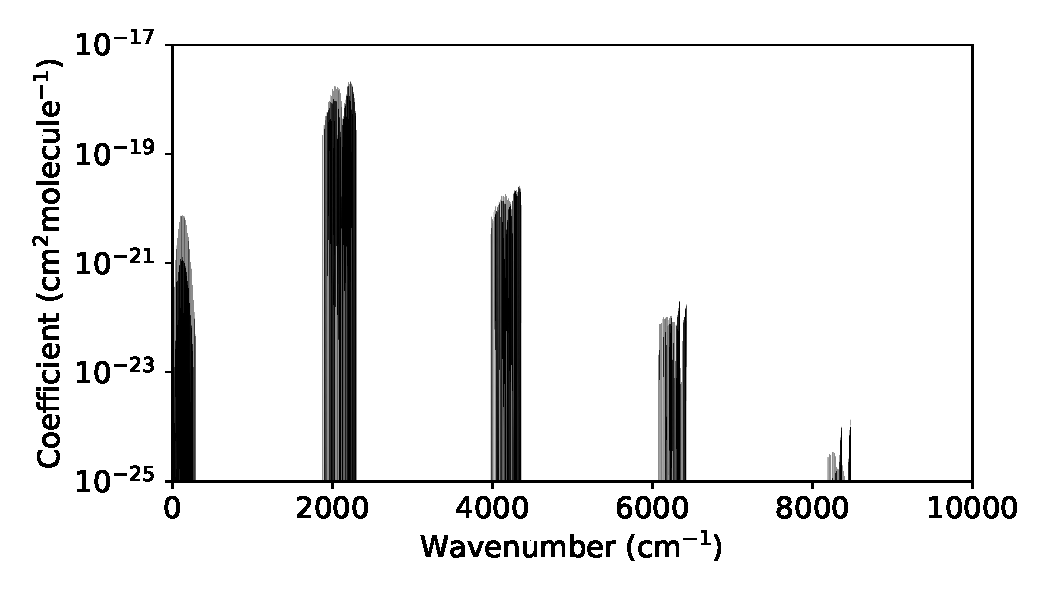
\includegraphics[width=0.85\textwidth]{figures/soc-lava-planets/co-absorption.pdf}
  \caption{The absorption coefficient of CO versus wavenumber at \SI{2500}{\kelvin} and \SI{1}{\bar} from the \textit{HITEMP} database \citep{rothman2010hitemp}. For the simulations in this chapter, the longwave radiation from the surface peaks at about \SI{5000}{\per\centi\metre} and the incoming stellar radiation peaks at about \SI{10000}{\per\centi\metre}, so the longwave optical depth of the CO-dominated atmospheres in this chapter is higher than the shortwave optical depth.}
  \label{fig:co-absorption}
\end{figure}

\subsection{Socrates Radiative Transfer}

Chapter \ref{ch:linking-climate-55cnce} used a semi-grey radiative transfer scheme to model the atmosphere of 55 Cancri e. This reduced the complexity and number of parameters of the model, but had two main limitations. First, the simple scheme may not fully represent the details of the real radiative transfer and global circulation. Second, the outgoing longwave radiation had no wavelength dependence in the model, so the \SI{4.5}{\micro\metre} radiation was post-processed by choosing a particular radiating level. This chapter will show how this approximation can be inaccurate, producing unrealistically large phase offsets in the thermal phase curve.

For the simulations in this chapter, I coupled the correlated-k radiative transfer scheme \textit{Socrates} \citep{edwards1996socrates} to Exo-FMS. This scheme represents the wavelength-dependent radiative effects of real gases, unlike the wavelength-independent semi-grey model. The simulations used low-resolution spectral data, and were then post-processed using higher-resolution data to produce simulated observations.

The \textit{Socrates} radiative transfer scheme requires a ``spectral file'' of gaseous absorption data to be generated from line lists. The simulations in this chapter generated this data from line lists in the \textit{HITEMP} database \citep{rothman2010hitemp}, using the utilities provided with the \textit{Socrates} code \citep{edwards1996socrates}. Figure \ref{fig:co-absorption} shows the absorption spectrum of CO, which was used to produced \textit{Socrates} spectral files for the simulations.


%%%%%%%%%%%%%%%%%%%%%%%%%%%%%%%%%%%%
\section{Control Simulation Results}\label{sec:control-simulations}

This section discusses two control simulations in the updated model, based on the first two tests using the previous model in Chapter \ref{ch:linking-climate-55cnce}. The first control simulation is Test 1, with a 10 bar H$_{2}$ atmosphere and a $1\%$ molar concentration of CO. The second simulation, Test 2, has a 10 bar N$_{2}$ atmosphere with a $1\%$ molar concentration of CO. The small amounts of CO were not taken into account when calculating the heat capacity of the atmosphere, to keep the bulk thermodynamic properties the same as the equivalent previous tests. Only absorption from CO is considered in the tests, to keep the radiative properties of the atmosphere the same. In reality, collision-induced absorption from H$_{2}$ and N$_{2}$ would also contribute to the opacity of the atmosphere.

% The choice of atmospheric composition is somewhat arbitrary and is designed to focus on the effect of the bulk composition on the circulation, and the effect of non-grey radiative transfer.

 It is not clear what gases are likely to make up the atmosphere of a lava planet. \citet{miguel2018observability} modelled N$_{2}$-dominated atmospheres with absorbers such as CO, CO$_{2}$, and H$_{2}$O. \citet{ito2015theoretical} modelled atmospheres of the rock vapour such as SiO that would be outgassed by a magma ocean. I will investigate the effect of an atmospheric opacity dominated by CO, which is a physically plausible gas with a strong longwave opacity. The modelling in this chapter does not aim to test the hypothesis that there is an atmosphere with exactly this composition on 55 Cancri e, but rather to show the effect of different atmospheric opacities at different wavelengths on the observed phase curve.

% The simulated observations were produced by running the radiative transfer scheme once at a higher resolution, and recording the outgoing radiation.

This section will compare the global circulation and temperature distribution of the two control tests to the equivalent tests in Chapter \ref{ch:linking-climate-55cnce} to determine if the non-grey radiative transfer makes a significant difference. I will then discuss the features of the emission spectra and thermal phase curves, and show how the radiative properties of the atmosphere can be degenerate with the strength of the circulation. I will conclude that the realistic radiative transfer does not greatly affect the global circulation in each test, but does strongly affect the observed thermal phase curve. I will follow these control tests with a ``best-fit'' case based on similar tests in Chapter \ref{ch:linking-climate-55cnce}.


 % It is important to note that the aim is not to exactly test the hypothesis that CO is the only absorber on the planet, but instead to investigate the effect of more realistic radiative transfer in general, particularly the effect of different atmospheric opacities on the observed phase curve. I therefore suggest that the conclusions apply generally to any atmosphere without an extreme longwave or shortwave opacity, and should be useful in interpresting the thermal phase curve whatever the real composition.

% It is not clear what gases are appropriate absorbers for the atmosphere of a lava planet, given the lack of observational characterisation. Hot Jupiter atmospheres are normally modelled with a variable metallicity \citep{amundsen2016hd209}, but the different formation pathways expected for the atmosphere of a terrestrial planet makes its composition less well constrained \citep{madhusudhan2016exoplanetary}. \citet{miguel2018observability} modelled N$_{2}$-dominated atmospheres with absorbers such as CO, CO$_{2}$, and H$_{2}$O. \citet{ito2015theoretical} modelled atmospheres of rock vapour such as SiO outgassed by a hypothetical magma ocean. In this chapter, I investigate the effect of an atmospheric opacity dominated by CO, as a physically plausible strong longwave absorber.
%
% 55 Cancri e is terrestrial and has been suggested to be carbon-rich \citep{madhusudhan2012possible}, so CO or CO$_{2}$ are reasonable candidates for atmospheric absorbers. CO$_{2}$ would tend to disproportionate in to CO at these high temperatures \citep{moses2014chemical}, so in this chapter I will only consider the effect of CO.




\subsection{Global Circulation}

\begin{figure}
  \centering
  \begin{subfigure}[t]{0.48\textwidth}
    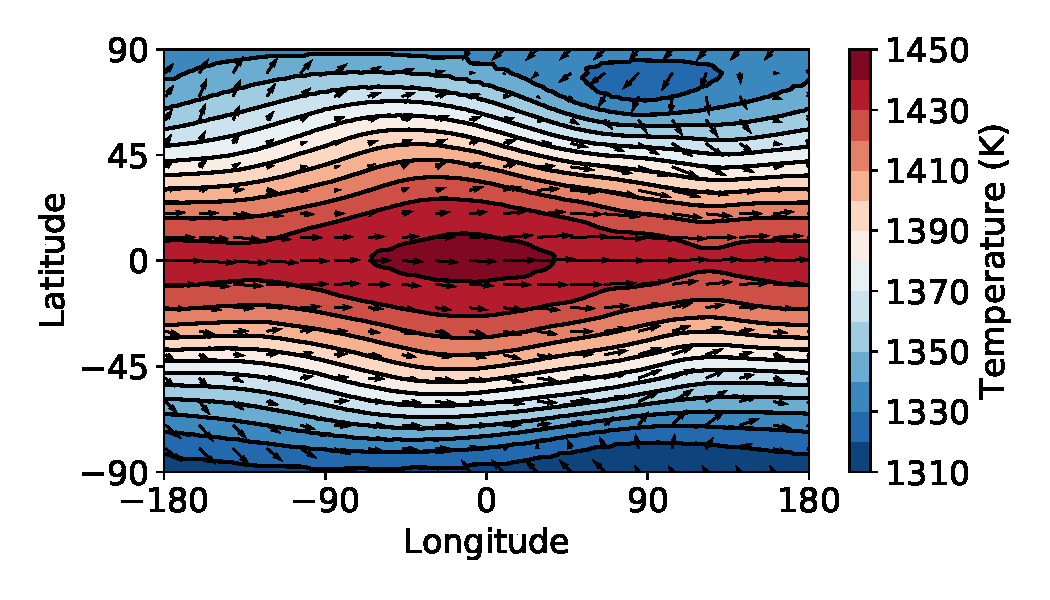
\includegraphics[width=\textwidth]{figures/soc-lava-planets/h2-soc-temp.pdf}
    \caption{Test 1: 10 bar H$_{2}$ atmosphere.}\label{fig:soc-temp-h2}
  \end{subfigure}
\quad
  \begin{subfigure}[t]{0.48\textwidth}
    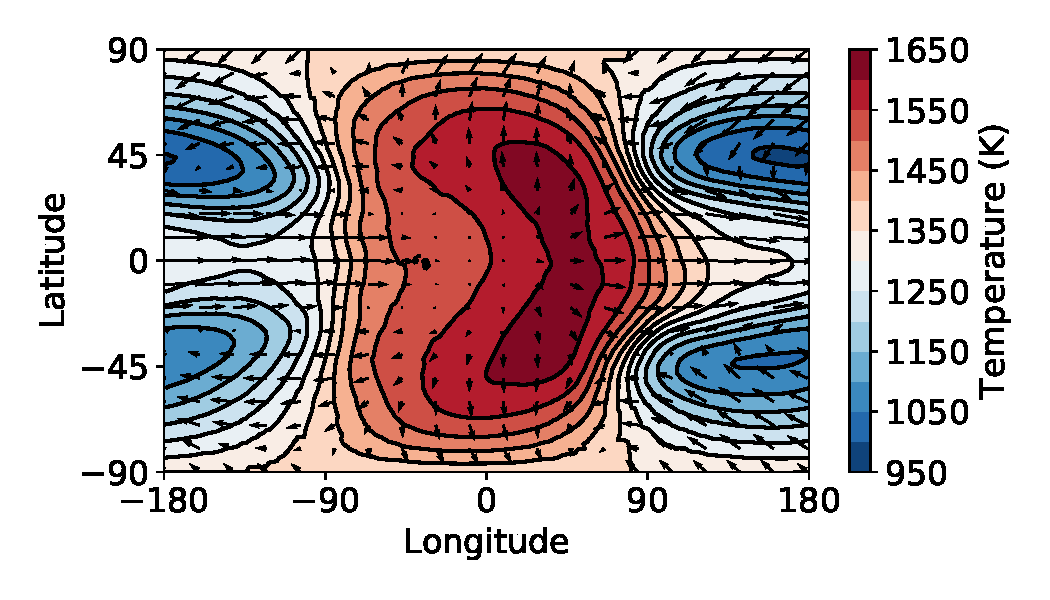
\includegraphics[width=\textwidth]{figures/soc-lava-planets/n2-soc-temp.pdf}
    \caption{Test 2: 10 bar N$_{2}$ atmosphere.}\label{fig:soc-temp-n2}
  \end{subfigure}
  \caption{Global temperature maps at the \SI{3.57}{\bar} pressure level of the simulations with $1\%$ CO. The mean molecular weight of the atmosphere affects the circulation and temperature distribution in the same way as in Chapter \ref{ch:linking-climate-55cnce}.}
  \label{fig:soc-temp}
\end{figure}

The model results shown in this chapter were time-averaged over either 100 or 200 days, after the model was spun up for at least 100 days. The model reached equilibrium well before 100 days according to the same conditions as in the previous chapter. Figure \ref{fig:soc-temp} shows the temperature fields at the pressure level corresponding to the position of the maximum zonal-mean zonal flow of Test 2. This is the level where the effect of the equatorial jet should be strongest. The tests have similar temperature distributions to the equivalent 10 bar H$_{2}$ and N$_{2}$ tests in Chapter \ref{ch:linking-climate-55cnce}, suggesting that the realistic radiative transfer in the new tests does not greatly change the global circulation compared to the previous simulations.


Test 2 has a large day-night contrast due to its high mean molecular weight and short radiative timescale, just like the equivalent test in the previous chapter. Test 1 has a more zonally uniform temperature field due to its low mean molecular weight and long radiative timescale, which is also in agreement with the semi-grey tests. Chapter \ref{ch:wave-mean-flow} explains why the radiative timescale affects the global temperature distribution.


Figure \ref{fig:soc-zonal-u} shows the zonal-mean zonal wind for Tests 1 and 2. The theory in Chapter \ref{ch:eqm-zonal-flow} correctly predicts that the more strongly damped Test 2 should have strong eastward flow at the equator and strong westward flow at high latitudes. Chapter \ref{ch:eqm-zonal-flow} also correctly predicts that the more weakly damped Test 1 should have weaker westward flow at high latitudes. It is not clear why there are two eastward jets at the equator in Test 1, which merits further investigation.

\begin{figure}
  \centering
  \begin{subfigure}[t]{0.48\textwidth}
    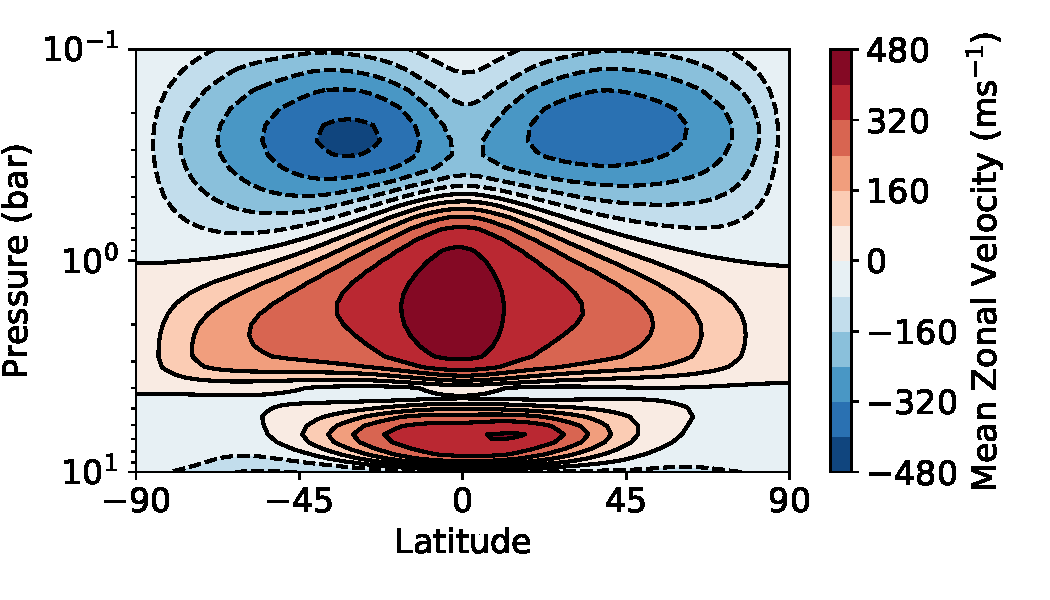
\includegraphics[width=\textwidth]{figures/soc-lava-planets/h2-soc-zonal-u.pdf}
    \caption{Test 1: 10 bar H$_{2}$ atmosphere.}\label{fig:soc-zonal-u-h2}
  \end{subfigure}
\quad
  \begin{subfigure}[t]{0.48\textwidth}
    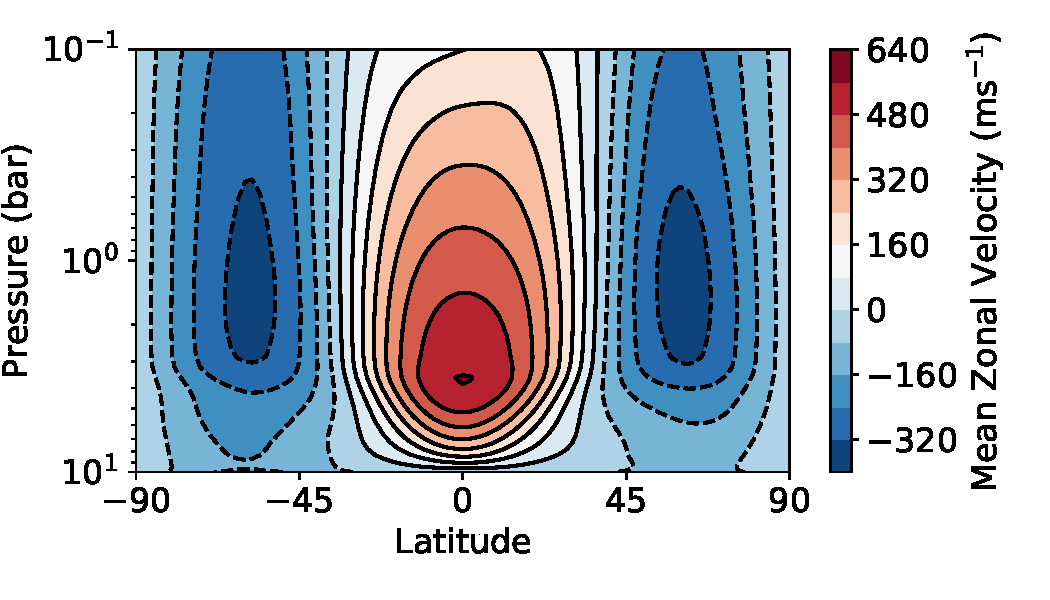
\includegraphics[width=\textwidth]{figures/soc-lava-planets/n2-soc-zonal-u.pdf}
    \caption{Test 2: 10 bar N$_{2}$ atmosphere.}\label{fig:soc-zonal-u-n2}
  \end{subfigure}
  \caption{Zonal-mean zonal wind of the simulations with $1\%$ CO. The strong westward flow at high latitudes in Test 2 is due to its strong radiative damping.}
  \label{fig:soc-zonal-u}
\end{figure}

Figure \ref{fig:soc-tp} shows temperature profiles of atmospheric columns in the model spaced evenly around the equators of Tests 1 and 2. The atmospheric temperature of Test 1 is almost uniform around the equator, except for pressure levels very near the surface, due to the long radiative timescale and efficient heat redistribution. Test 2 has weaker heat redistribution due to its short radiative timescale caused by its higher mean molecular weight, so the day-side and night-side temperature profiles are very different. These profiles are qualitatively similar to the equivalent tests in Chapter \ref{ch:linking-climate-55cnce}.

\begin{figure}
  \centering
  \begin{subfigure}[t]{0.49\textwidth}
    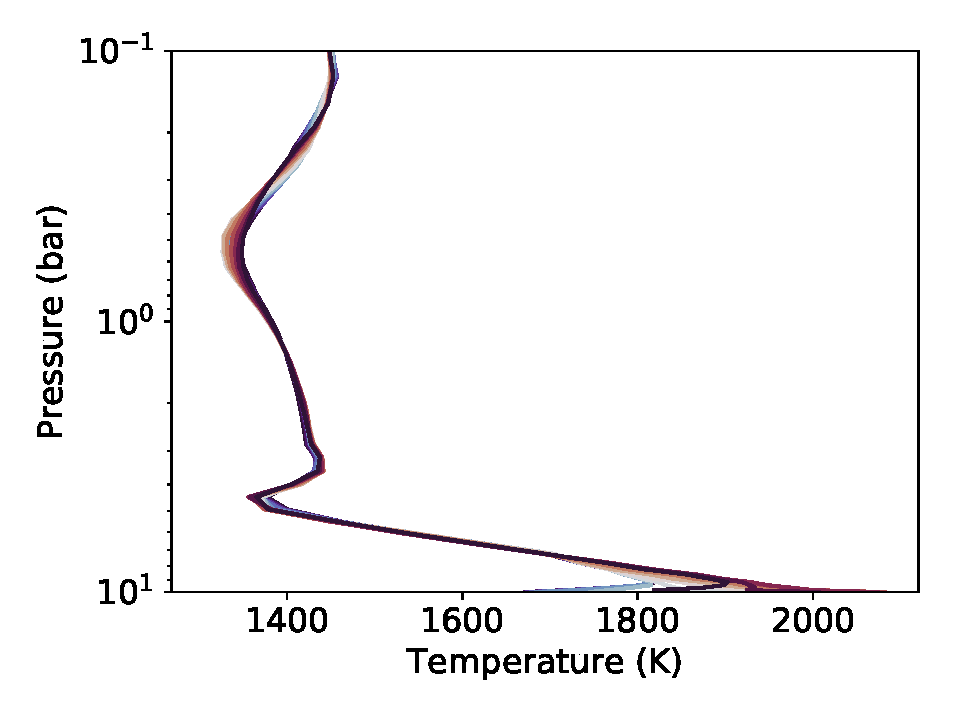
\includegraphics[width=\textwidth]{figures/soc-lava-planets/h2-soc-tp.pdf}
    \caption{Test 1: 10 bar H$_{2}$ atmosphere.}\label{fig:soc-tp-h2}
  \end{subfigure}
  %
  \begin{subfigure}[t]{0.49\textwidth}
    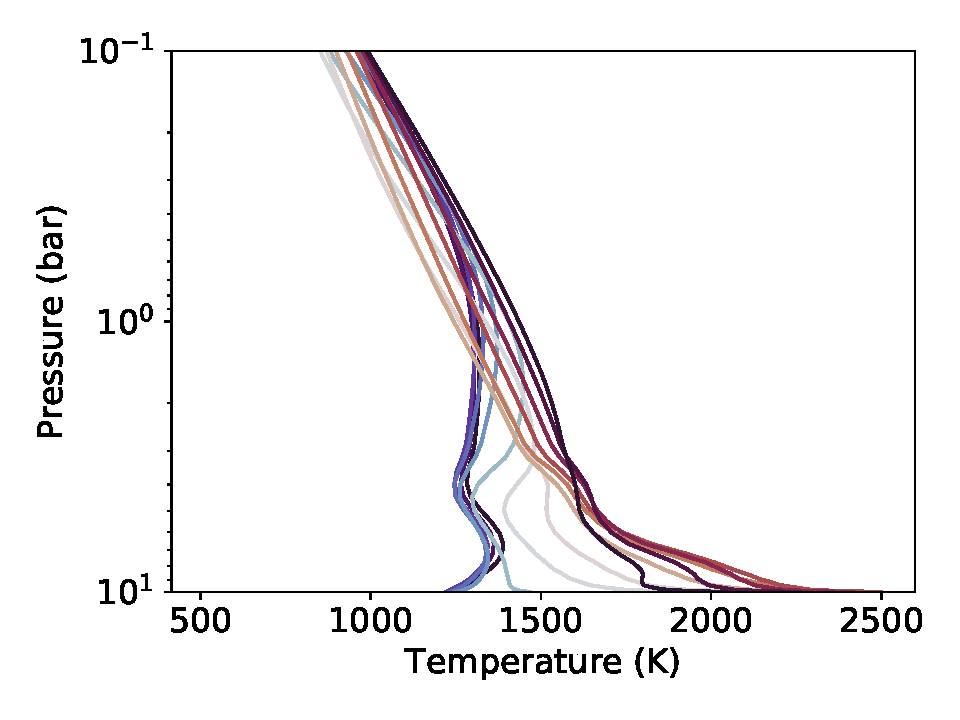
\includegraphics[width=\textwidth]{figures/soc-lava-planets/n2-soc-tp.pdf}
    \caption{Test 2: 10 bar N$_{2}$ atmosphere.}\label{fig:soc-tp-n2}
  \end{subfigure}
  \caption{Temperature profiles of the simulations with $1\%$ CO. Test 1 has much more efficient heat circulation than Test 2, so its temperature profiles are almost homogeneous.}
  \label{fig:soc-tp}
\end{figure}

The similarity of the global circulation and temperature structure of these tests to the corresponding tests in the previous chapter suggests that the more realistic radiative transfer does not strongly affect the atmospheric dynamics. This means that the idealised semi-grey model is still useful to investigate the global circulation of these planets. More realistic radiative transfer might be required to model atmospheres with radiative features such as strong shortwave absorption or variable albedo, which could be caused by heterogeneous composition or cloud formation.

% In summary, these control tests suggest that the scaling relations and conclusions of Chapter \ref{ch:linking-climate-55cnce} still apply in this new model with more realistic radiative transfer.


\subsection{Thermal Emission}

This section shows the outgoing longwave radiation and emission spectra produced by post-processing the final state of each test with a higher-resolution spectral file with 621 bands. Hemisphere-averaged spectra and phase curves were produced with the STARRY software package \citep{luger2019starry}. Figure \ref{fig:soc-spec-olr} shows the spectral radiance of the outgoing longwave radiation in Tests 1 and 2, from columns evenly spaced around the equator at the substellar point, east terminator, antistellar point, and west terminator. Each spectrum shows the three main CO absorption features in this range, at 2000, 4000, and \SI{6000}{\per\centi\metre}.

The differences between the OLR of Tests 1 and 2 are only due to their global circulation and the resulting temperature distribution, as they have the same surface pressure and mixing ratio of CO. The substellar and antistellar OLR are closer in magnitude in Test 1 than in Test 2, due to the higher day-night contrast in Test 2 discussed above. The eastward heat circulation in Test 1 warms the east terminator, so the emission there is greater than the emission from the west terminator. This effect is reversed in Test 2, where the stationary wave response temperature field in Test \ref{fig:soc-temp} is not shifted by the zonal flow due to the short radiative timescale (giving a wave pattern similar to the response to forcing in \citet{matsuno1966quasi}). This means that the west terminator is warmer (as the unshifted stationary wave response is stronger there), making the OLR at the west terminator stronger than that at the east terminator. Observations of spectrally resolved phase curves may reveal dynamical effects like this in the future \citep{stevenson2014thermal}.


% Test 1 has a substellar surface temperature of about \SI{2300}{\kelvin} and an anti-stellar temperature of about\SI{1800}{\kelvin}, while Test 2 has a substellar temperature of about \SI{2500}{\kelvin} and an antistellar temperature of about \SI{1700}{\kelvin}.



\begin{figure}
  \centering
  \begin{subfigure}[t]{0.48\textwidth}
    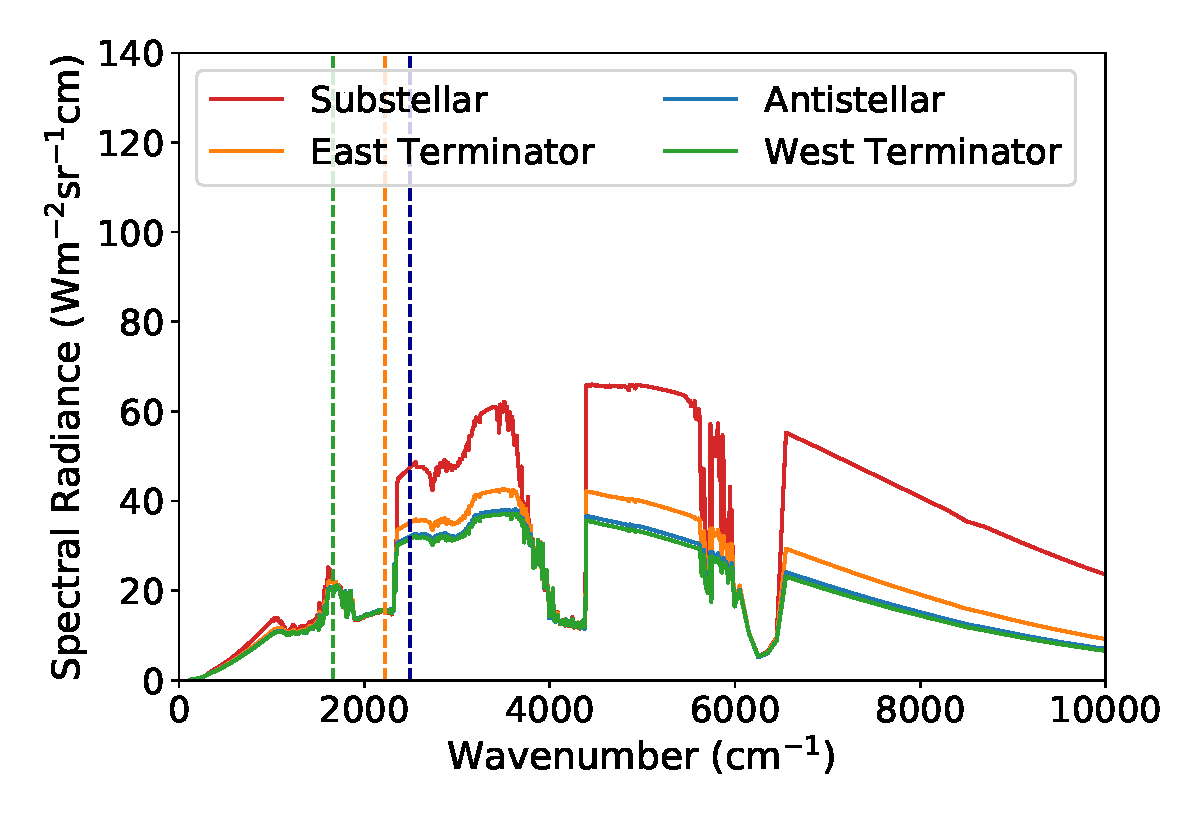
\includegraphics[width=\textwidth]{figures/soc-lava-planets/h2-spec-olr.pdf}
    \caption{Test 1: 10 bar H$_{2}$ atmosphere.}\label{fig:soc-spec-olr-h2}
  \end{subfigure}
\quad
  \begin{subfigure}[t]{0.48\textwidth}
    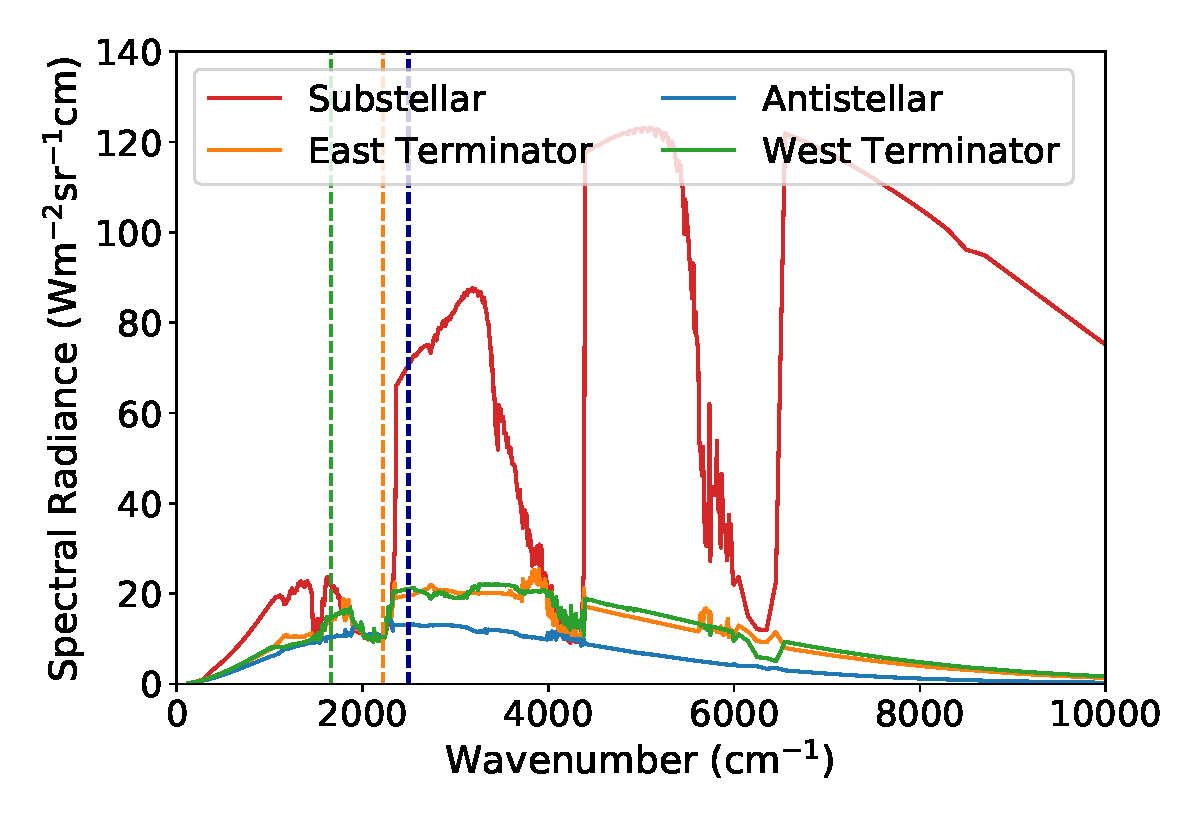
\includegraphics[width=\textwidth]{figures/soc-lava-planets/n2-spec-olr.pdf}
    \caption{Test 2: 10 bar N$_{2}$ atmosphere.}\label{fig:soc-spec-olr-n2}
  \end{subfigure}
  \caption{Spectral radiance of the outgoing longwave radiation (OLR) of Tests 1 and 2, showing the main CO absorption features at 2000, 4000, and \SI{6000}{\per\centi\metre}. The relative magnitudes of the fluxes at each longitude are due to the instellation and global circulation.}
  \label{fig:soc-spec-olr}
\end{figure}

Figure \ref{fig:soc-emission-spec} shows simulated emission spectra of the day-sides and night-sides of Tests 1 and 2. These contain the same information as the plots in Figure \ref{fig:soc-spec-olr}, but the emission spectra are averaged over the hemisphere and divided by the stellar flux at that wavelength. The vertical dashed lines show the wavelengths of the phase curves plotted later in Figure \ref{fig:soc-spec-pc}, and the shaded region shows the extent of the \SI{4.5}{\micro\metre} \textit{Spitzer} bandpass used by \citet{demory201655cnce}.

The spectra show the same absorption features as Figure \ref{fig:soc-spec-olr}. Emission features could appear in these spectra given a temperature inversion, which would require a shortwave absorber high in the day-side atmosphere. The differences between the day-side and night-side emission spectra show the day-night contrast of each test, which is much larger in Test 2 than Test 1. These figures show the three-dimensional radiative and dynamical information contained in phase-resolved emission spectroscopy, which may be possible for lava planets like 55 Cancri e using upcoming telescopes such as ARIEL \citep{stevenson2014thermal, tinetti2016ariel}.


% The new radiative transfer scheme did not affect the global circulation greatly, but does affect the simulated observations due to the strong wavelength dependence.


\begin{figure}
  \centering
  \begin{subfigure}[t]{0.48\textwidth}
    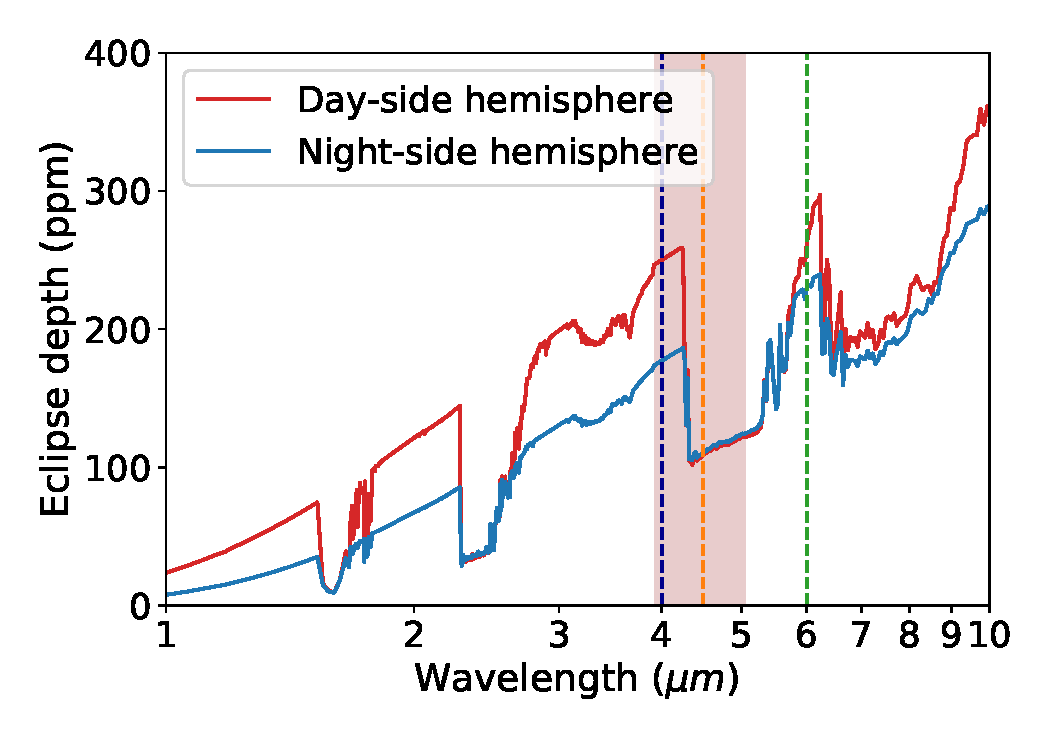
\includegraphics[width=\textwidth]{figures/soc-lava-planets/h2-emission-spec.pdf}
    \caption{Test 1: 10 bar H$_{2}$ atmosphere.}\label{fig:soc-tp-h2}
  \end{subfigure}
\quad
  \begin{subfigure}[t]{0.48\textwidth}
    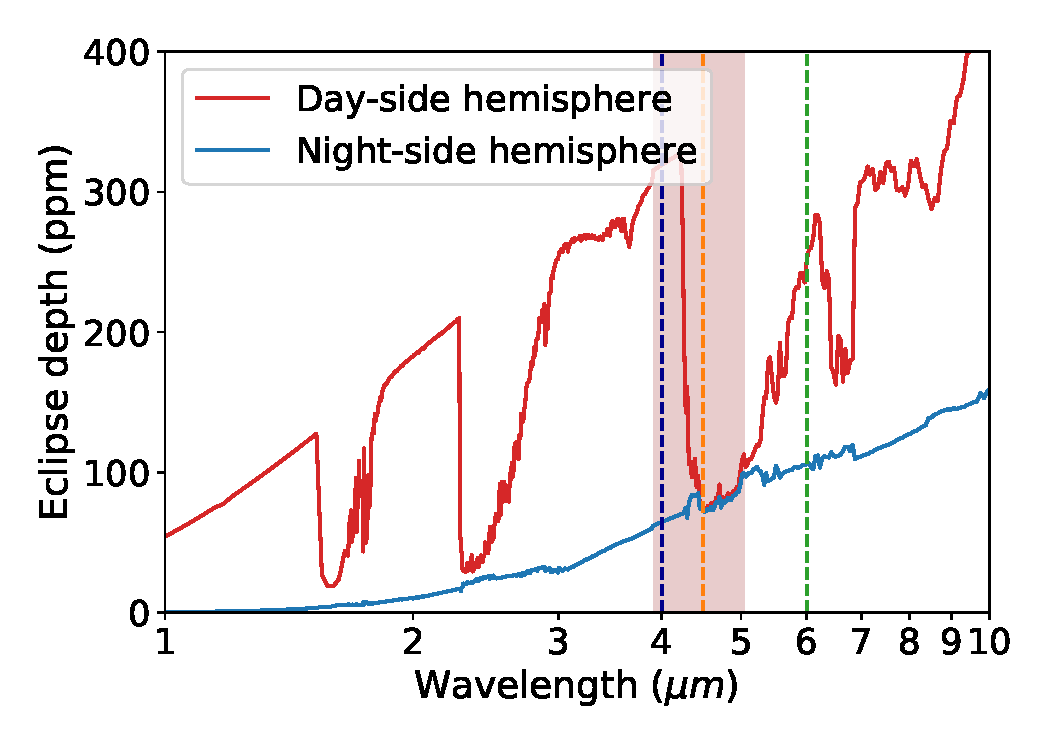
\includegraphics[width=\textwidth]{figures/soc-lava-planets/n2-emission-spec.pdf}
    \caption{Test 2: 10 bar N$_{2}$ atmosphere.}\label{fig:soc-tp-n2}
  \end{subfigure}
  \caption{Emission spectra of the day-side and night-side of Tests 1 and 2, showing the CO absorption features. The day-night contrast varies with atmospheric opacity. The green, orange, and blue dashed lines show the wavelengths corresponding to the phase curves of the same colours in Figure \ref{fig:soc-spec-pc}.}
  \label{fig:soc-emission-spec}
\end{figure}


\subsection{Thermal Phase Curves}

Figure \ref{fig:soc-spec-pc} shows thermal phase curves calculated from snapshots of the thermal emission of Tests 1 and 2 at a higher spectral resolution. Figure \ref{fig:phase-curve-diagram} showed that the phase curve is the hemisphere-integrated emission from the planet as a function of orbital phase. Note that the phase curves in this chapter are plotted by orbital phase rather than planetary longitude, so are reversed compared to the simulated phase curve in Chapter \ref{ch:linking-climate-55cnce}. The thick black line in Figure \ref{fig:soc-spec-pc} is the phase curve measured by \citet{demory201655cnce}, with a hot-spot shift of \ang{41} east of the substellar point, and a day-night contrast of \SI{1300}{\kelvin}. The observed phase curve contains the primary and secondary eclipses at phases of 0 and $\pi$, unlike those calculated from the simulations.

The colours of the other phase curves correspond to the wavelengths shown by the dashed lines of the same colours in Figure \ref{fig:soc-emission-spec}. The atmospheric opacity at the wavelength of the phase curve determines the contributions of each pressure level to the thermal emission, making the phase curve depend strongly on the wavelength observed. This is similar to the effect of varying the radiating level in Chapter \ref{ch:linking-climate-55cnce}. A phase curve at a low atmospheric opacity or at a radiating level close to the surface will have a large day-night contrast, and vice versa. The thick red lines shows the phase curves that would be observed in the \textit{Spitzer} \SI{4.5}{\micro\metre} bandpass. They are weighted by the response function of the IRAC\footnote{The Infrared Array Camera, with a response function available at \url{irsa.ipac.caltech.edu/data/SPITZER/docs/irac/calibrationfiles/spectralresponse}} instrument, which corresponds to the band shaded in red in Figure \ref{fig:soc-emission-spec}.


\begin{figure}
  \centering
  \begin{subfigure}[t]{0.49\textwidth}
    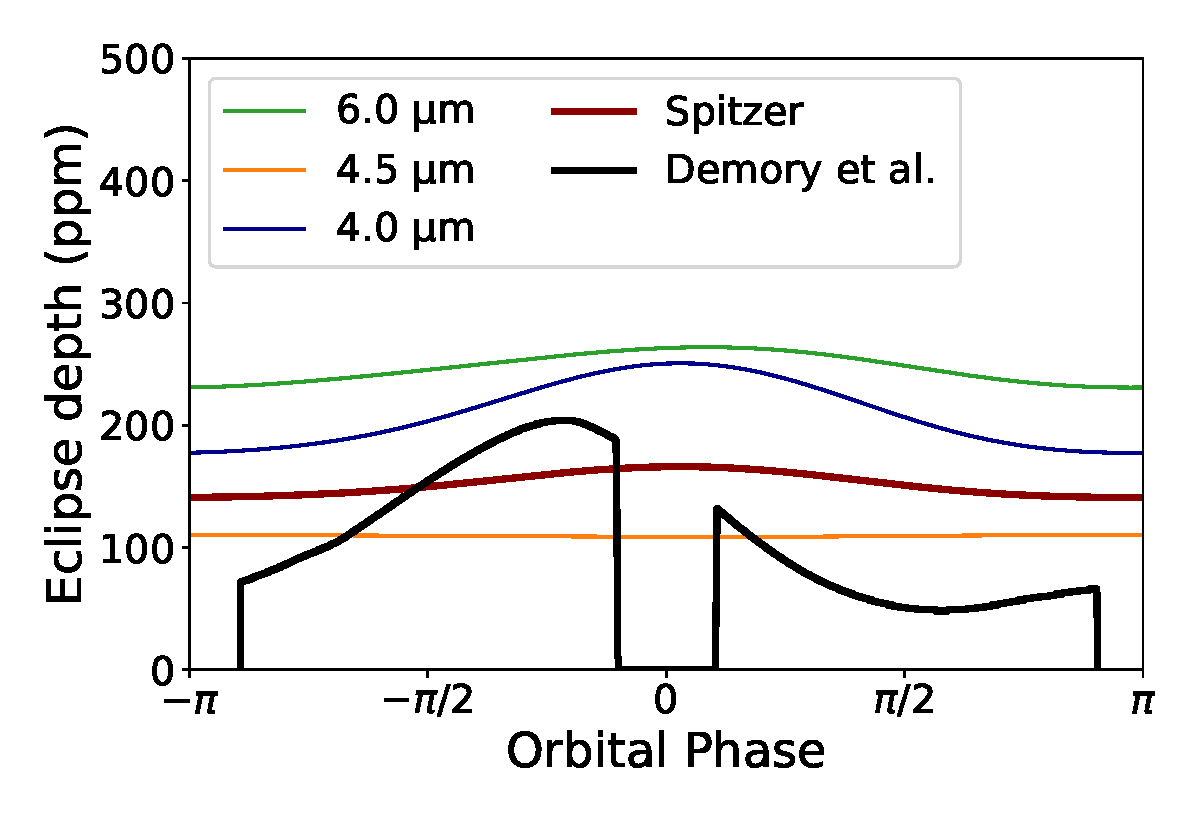
\includegraphics[width=\textwidth]{figures/soc-lava-planets/h2-spec-pc.pdf}
    \caption{Test 1: 10 bar H$_{2}$ atmosphere.}\label{fig:soc-spec-pc-h2}
  \end{subfigure}
  %
  \begin{subfigure}[t]{0.49\textwidth}
    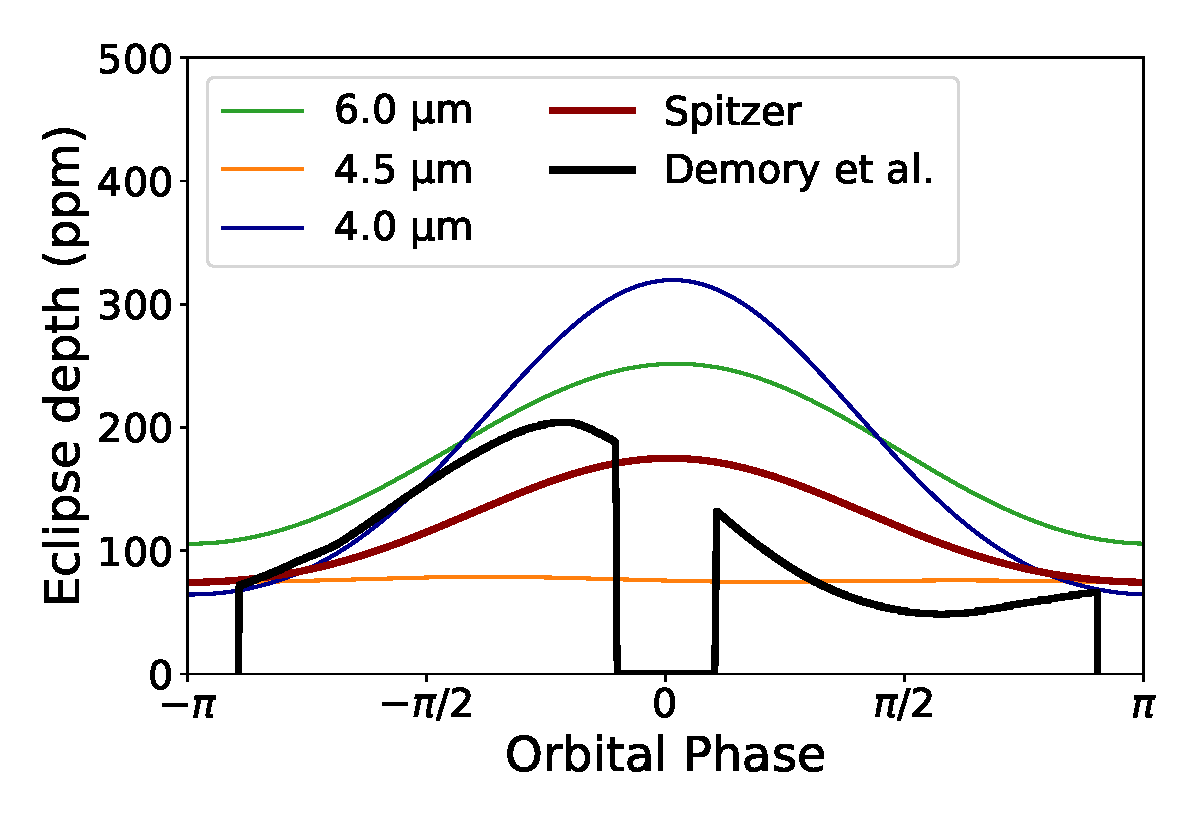
\includegraphics[width=\textwidth]{figures/soc-lava-planets/n2-spec-pc.pdf}
    \caption{Test 2: 10 bar N$_{2}$ atmosphere.}\label{fig:soc-spec-pc-n2}
  \end{subfigure}
  \caption{Thermal phase curves of Tests 1 and 2. The thick black line shows the phase curve observed by \citet{demory201655cnce} in the \textit{Spitzer} \SI{4.5}{\micro\metre} channel. The thick red line is the phase curve simulated from each test using the same \SI{4.5}{\micro\metre} bandpass. The other coloured lines show phase curves calculated at the wavelengths plotted in the same colours in Figure \ref{fig:soc-emission-spec}.}
  \label{fig:soc-spec-pc}
\end{figure}

None of the phase curves in Figure \ref{fig:soc-spec-pc} have a significant phase offset, despite the efficient heat redistribution in Test 1. The OLR is dominated by emission from the surface at most wavelengths. The surface temperature is closely coupled to the instellation, so there is normally no large phase shift in its emission. I will discuss the implications of this later in the chapter.

The day-night contrasts of the phase curves in Figure \ref{fig:soc-spec-pc} depend on both the mean molecular weight of the atmosphere, and the opacity of the atmosphere at the wavelength observed. The phase curves of Test 1 have smaller day-night contrasts in Test 2 due to the stronger heat circulation in Test 1; this is consistent with the results of Chapter \ref{ch:linking-climate-55cnce}. Larger day-night contrasts are also seen in the phase curves observed at wavelengths of lower opacity such as the blue \SI{4.0}{\micro\metre} curves, where the emission from the surface dominates the OLR. Conversely, the orange \SI{4.5}{\micro\metre} lines in both cases are almost flat as the OLR is from very high in the atmosphere where the temperature is almost uniform. The thick red line calculated in the \textit{Spitzer} bandpass observed by \citet{demory201655cnce} approximately matches the day-night contrast of the observations in Test 2, but does not match any of the features in Test 1.



% In both tests, the orange phase curve at \SI{4.5}{\micro\metre} has very small amplitudes, due to the high atmospheric opacity at this wavelength. This means that the radiating level is at a very low pressure, which has almost homogenous temperature due to the strong atmospheric circulation. Both tests also have phase curves with very large amplitude in the blue \SI{4.0}{\micro\metre} case. This is caused by the very low atmospheric opacity at this wavelength, so the phase curve corresponds to a high pressure, near the surface where the day-night contrast is large.


% This means that Test 2 is consistent with the equivalent 10 bar N$_{2}$ test in Chapter \ref{ch:linking-climate-55cnce}, which had no hot-spot shift or phase offset. However, it means that Test 1 is not consistent with the equivalent 10 bar H$_{2}$ test in Chapter \ref{ch:linking-climate-55cnce}, which had a large hot-spot shift in the temperature field. This is due first of all to the fact that the temperature field in Figure \ref{fig:soc-temp} is more zonally homogeneous than in the previous chapter. It also appears that the level of the jet, where there is some longitudinal variation of temperature),does not contribute greatly to the thermal emission, so this variation does not show up clearly. I will discuss this effect in more detail in the next section.




\subsection{Control Tests Summary}

The control tests using the updated model with the \textit{Socrates} radiative transfer scheme qualitatively matched the global circulation and temperature distribution of the corresponding tests in Chapter \ref{ch:linking-climate-55cnce}. This suggests that the semi-grey radiative transfer was a good approximation to the more realistic model in this chapter.

However, the simulated observations of Tests 1 and 2 were very different to the results of Chapter \ref{ch:linking-climate-55cnce}. The realistic radiative transfer showed that the phase curves depended strongly on the atmospheric opacity, and that this was degenerate with other properties such as mean molecular weight. Neither of the control tests matched the observed phase curve well, so in the next section I will discuss two tests that were designed to fit the observations more closely.


%%%%
%%%%%% TO HERE 24/09


%%%%%%%%%%%%%%%%%%%%%%%%%%%%%%%%%%%%
\section{Best-Fit Simulation Results}\label{sec:best-fit-simulation}

The control simulations did not match the observed phase curve. As in Chapter \ref{ch:linking-climate-55cnce}, their extreme mean molecular weights led to either too much heat redistribution, or too little. I therefore ran a new test similar to the ``best-fit'' simulation in the previous chapter with an intermediate mean molecular weight. This new test, Test 3, has a mixing ratio of 0.1 N$_{2}$ and 0.9 H$_{2}$. Its other parameters are the same as the two control tests, with a mixing ratio of 0.01 CO and a 10 bar surface pressure. The results of Test 3 are plotted as a time-average from 200 to 400 days.

This section shows its global circulation and simulated observations. I will show how the scaling relations from Chapter \ref{ch:linking-climate-55cnce} still describe the changes in global circulation compared to the control tests. However, the simulated observations will show that there is no observable phase offset in the thermal phase curve despite the hot-spot shift in the temperature field. I will suggest that this is because the surface pressure is too low, and in the next section will simulate a thicker atmosphere.


\begin{figure}
  \centering
  \begin{subfigure}[t]{0.48\textwidth}
    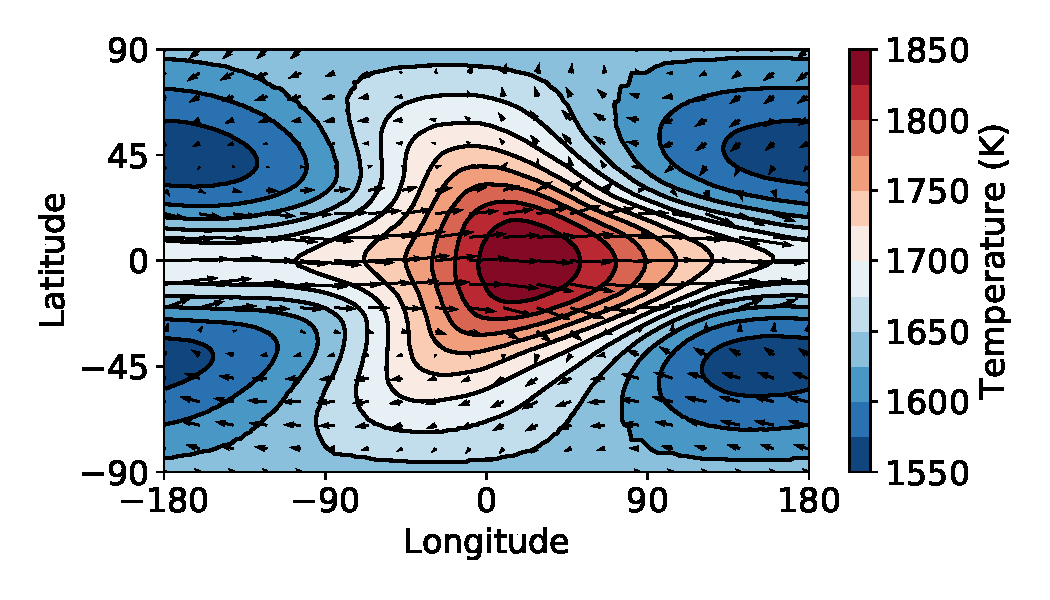
\includegraphics[width=\textwidth]{figures/soc-lava-planets/h2n2-soc-temp.pdf}
    \caption{Test 3: 10 bar mixed H$_{2}$-N$_{2}$ atmosphere.}\label{fig:soc-temp-h2n2}
  \end{subfigure}
\quad
  \begin{subfigure}[t]{0.48\textwidth}
    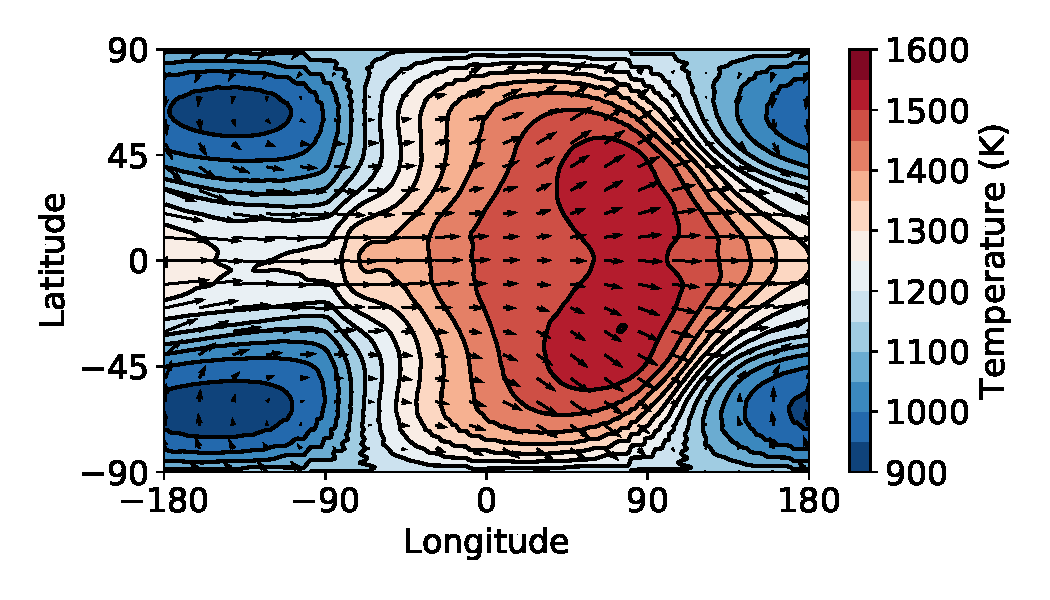
\includegraphics[width=\textwidth]{figures/soc-lava-planets/n2-100bar-soc-temp.pdf}
    \caption{Test 4: 100 bar N$_{2}$ atmosphere.}\label{fig:soc-temp-n2-100bar}
  \end{subfigure}
  \caption{Global temperature maps of Tests 3 and 4, at pressure levels chosen to show the largest hot-spot shift. Test 3 is plotted at the \SI{8.24}{\bar} pressure level, and has a small hot-spot shift that does not appear in the thermal phase curve. Test 4 is plotted at the \SI{28.3}{\bar} pressure level, and has a large hot-spot shift that appears in the thermal phase curve.}
  \label{fig:soc-temp-best}
\end{figure}


\subsection{Global Circulation}

Figure \ref{fig:soc-temp-h2n2} shows the global temperature field at the pressure level of the maximum zonal-mean zonal velocity for Test 3. It has a distinct hot-spot shift and day-night contrast due to its intermediate mean molecular weight, like the best-fit test in Chapter \ref{ch:linking-climate-55cnce}. The hot-spot shift is smaller than that of the test in Chapter \ref{ch:linking-climate-55cnce}, possibly due to the different radiative transfer scheme in this chapter, but should still affect the thermal emission from the layer of the jet. Figure \ref{fig:soc-zonal-u-h2n2} shows the zonal-mean zonal flow, with a single eastward equatorial jet that produces the hot-spot shift. The westward flow at high latitudes is weaker than Test 2 but stronger than Test 1. This is consistent with the predictions of Chapter \ref{ch:eqm-zonal-flow}, as its radiative damping timescale is shorter than Test 1 but longer than Test 2.


\begin{figure}
  \centering
  \begin{subfigure}[t]{0.48\textwidth}
    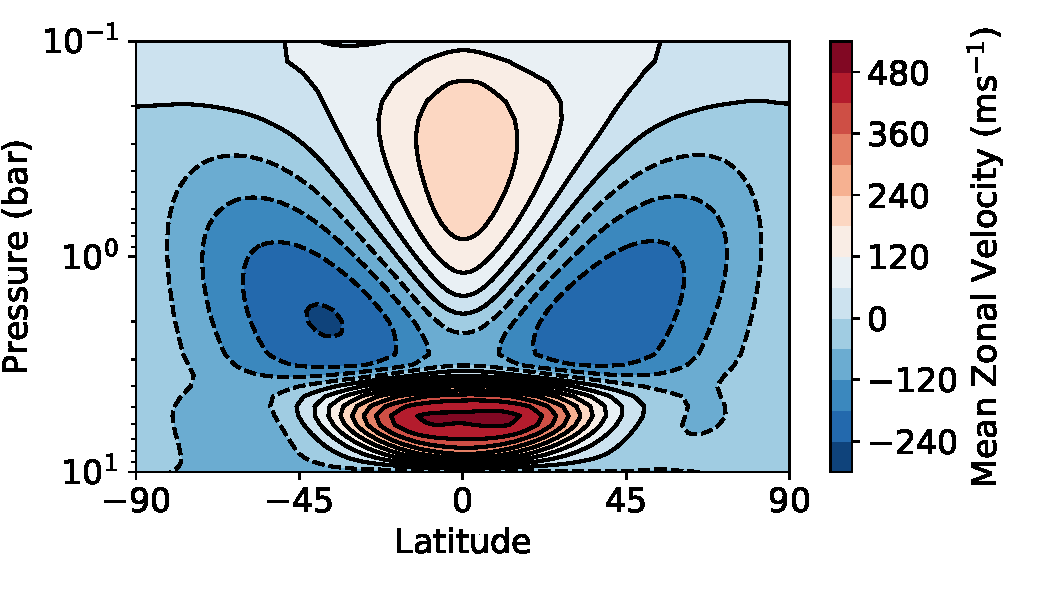
\includegraphics[width=\textwidth]{figures/soc-lava-planets/h2n2-soc-zonal-u.pdf}
    \caption{Test 3: 10 bar mixed H$_{2}$-N$_{2}$ atmosphere.}\label{fig:soc-zonal-u-h2n2}
  \end{subfigure}
\quad
  \begin{subfigure}[t]{0.48\textwidth}
    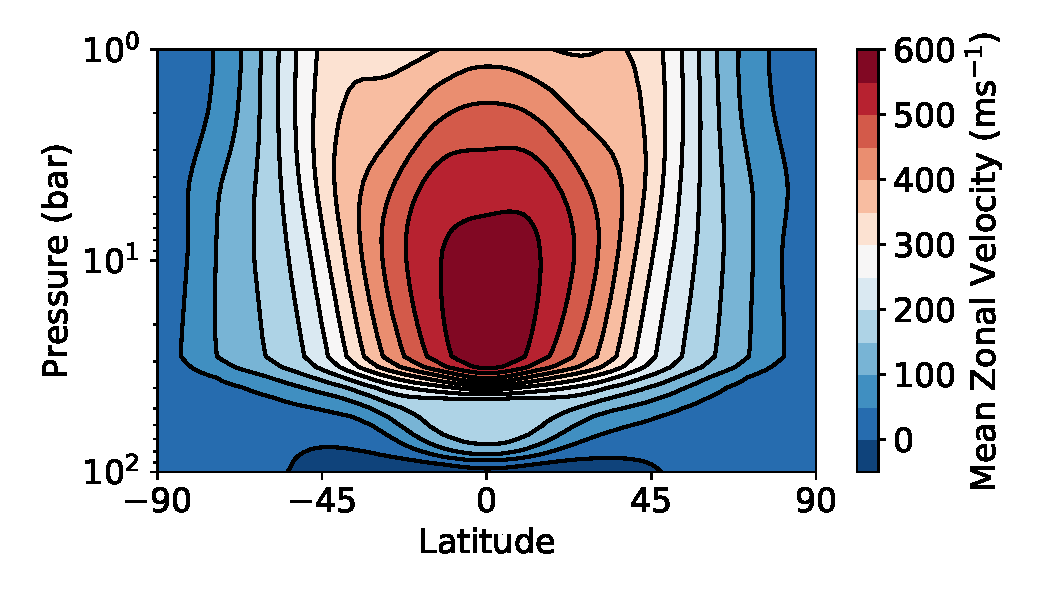
\includegraphics[width=\textwidth]{figures/soc-lava-planets/n2-100bar-soc-zonal-u.pdf}
    \caption{Test 4: 100 bar N$_{2}$ atmosphere.}\label{fig:soc-zonal-u-n2-100bar}
  \end{subfigure}
    \caption{Zonal-mean zonal wind of Tests 3 and 4, showing an equatorial jet produced by longwave heating in Test 3 and a similar jet produced mostly by shortwave heating in Test 4.}
  \label{fig:soc-zonal-wind-best}
\end{figure}

Figure \ref{fig:soc-tp-h2n2} shows the temperature profiles around the equator of Test 3. There is more day-night variation than Test 1 and less day-night variation than Test 2, as expected from the intermediate radiative timescale. The global circulation and resulting temperature distribution is similar overall to the corresponding best-fit test with semi-grey radiative transfer in Chapter \ref{ch:linking-climate-55cnce}.

\begin{figure}
  \centering
  \begin{subfigure}[t]{0.49\textwidth}
    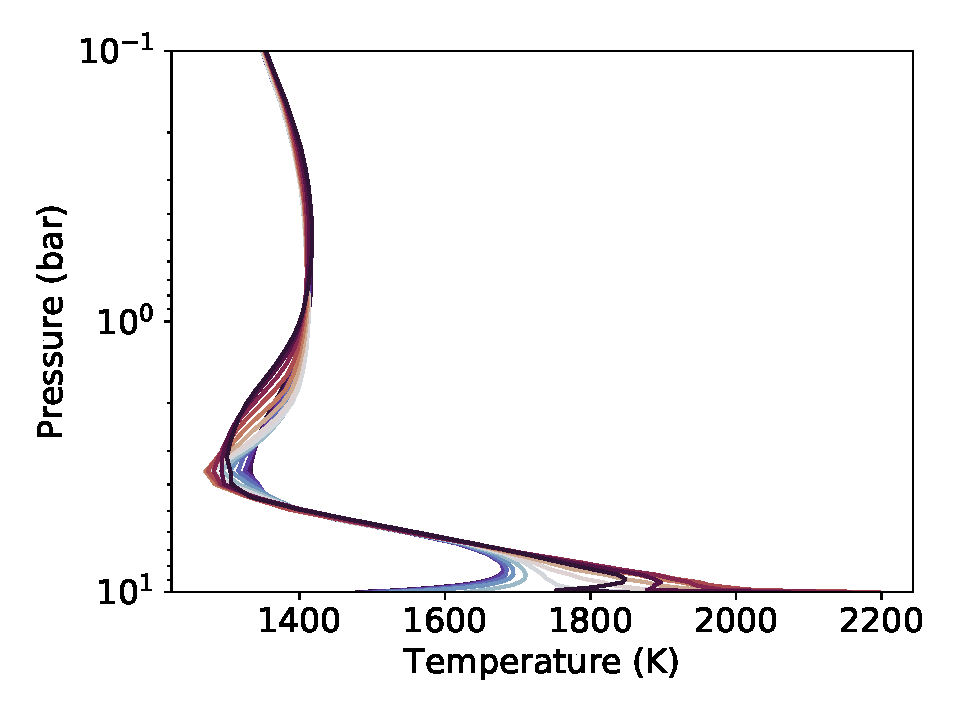
\includegraphics[width=\textwidth]{figures/soc-lava-planets/h2n2-soc-tp.pdf}
    \caption{Test 3: 10 bar mixed H$_{2}$-N$_{2}$ atmosphere.}\label{fig:soc-tp-h2n2}
  \end{subfigure}
  %
  \begin{subfigure}[t]{0.49\textwidth}
    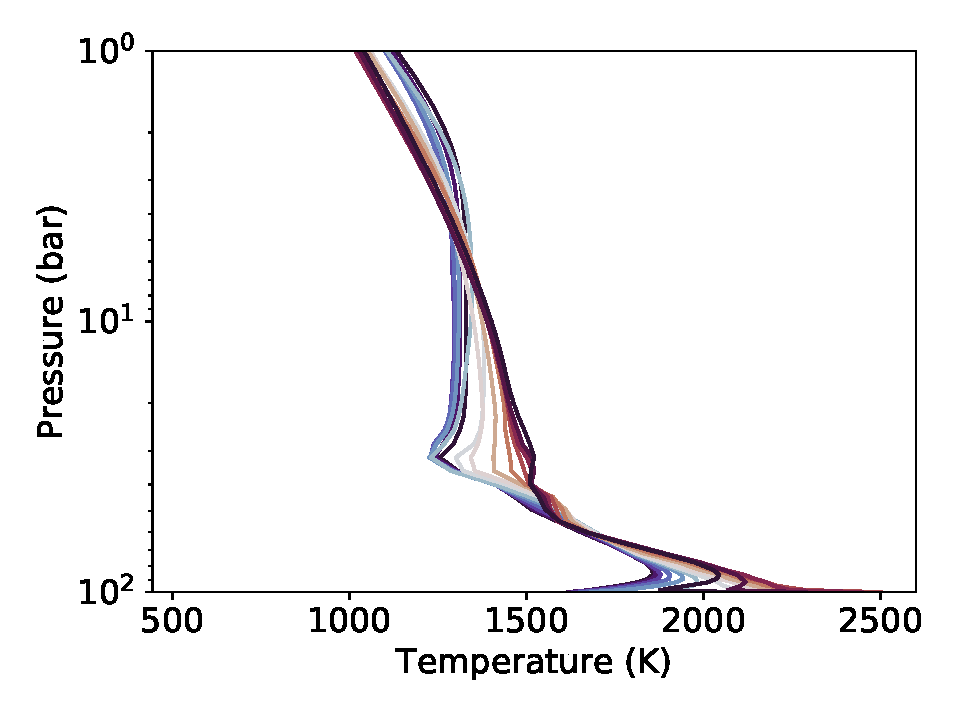
\includegraphics[width=\textwidth]{figures/soc-lava-planets/n2-100bar-soc-tp.pdf}
    \caption{Test 4: 100 bar N$_{2}$ atmosphere.}\label{fig:soc-tp-n2-100bar}
  \end{subfigure}
  \caption{Temperature profiles around the equators of Tests 3 and 4, showing the moderate day-night variation in Test 3 and the greater day-side heating due to shortwave absorption in Test 4.}
  \label{fig:soc-tp-best}
\end{figure}


% \begin{figure}
%   \centering
%     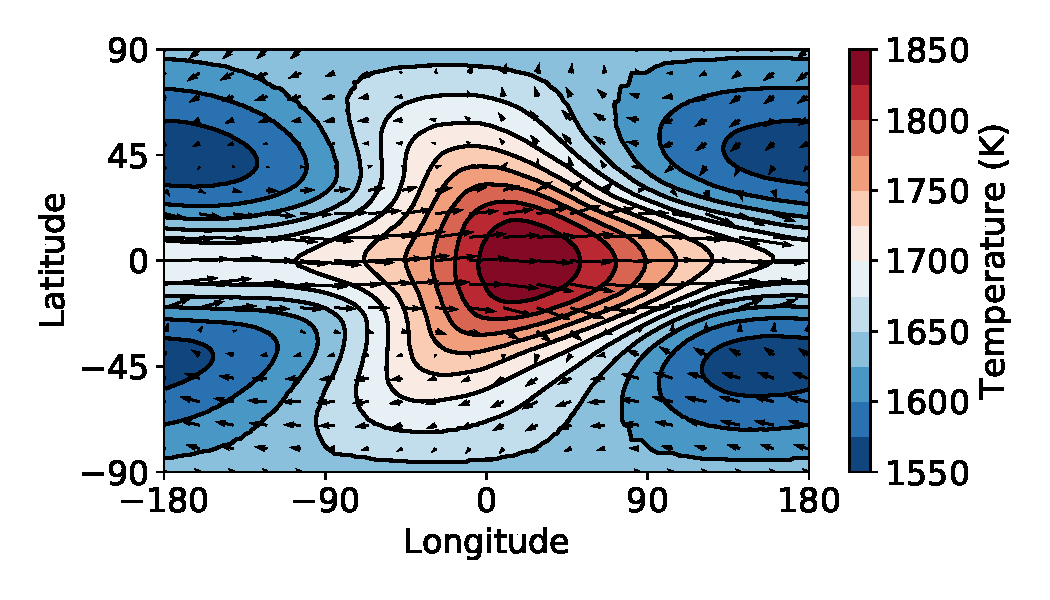
\includegraphics[width=0.49\textwidth]{figures/soc-lava-planets/h2n2-soc-temp.pdf}
%     \caption{Global temperature maps of the 10 bar mixed H$_{2}$-N$_{2}$ test at the X pressure level.}\label{fig:soc-temp-h2n2}
% \end{figure}


% \begin{figure}
%   \centering
%     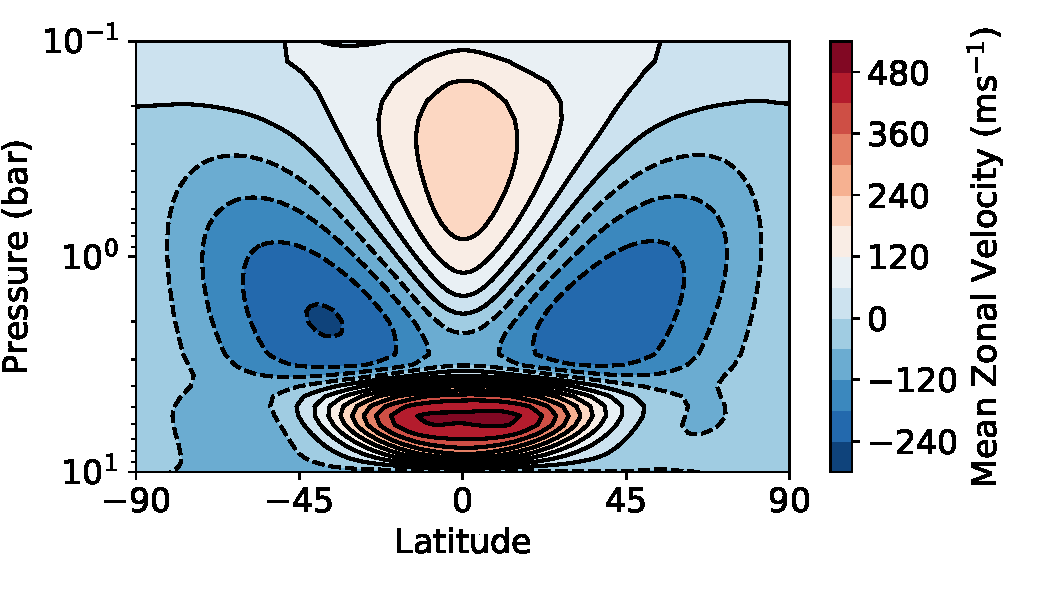
\includegraphics[width=0.49\textwidth]{figures/soc-lava-planets/h2n2-soc-zonal-u.pdf}
%     \caption{Zonal-mean zonal wind of the 10 bar mixed H$_{2}$-N$_{2}$ test.}\label{fig:soc-zonal-u-h2n2}
% \end{figure}



% \begin{figure}
%   \centering
%     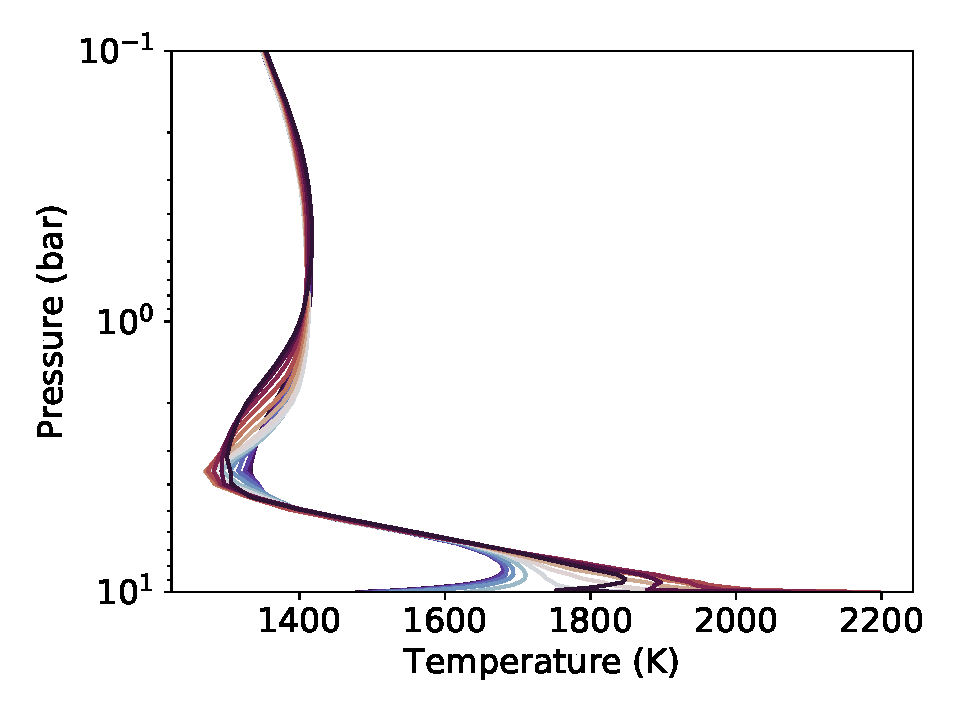
\includegraphics[width=0.49\textwidth]{figures/soc-lava-planets/h2n2-soc-tp.pdf}
%     \caption{Temperature profiles of the 10 bar mixed H$_{2}$-N$_{2}$ test.}\label{fig:soc-tp-h2n2}
% \end{figure}

\begin{figure}
  \centering
  \begin{subfigure}[t]{0.49\textwidth}
    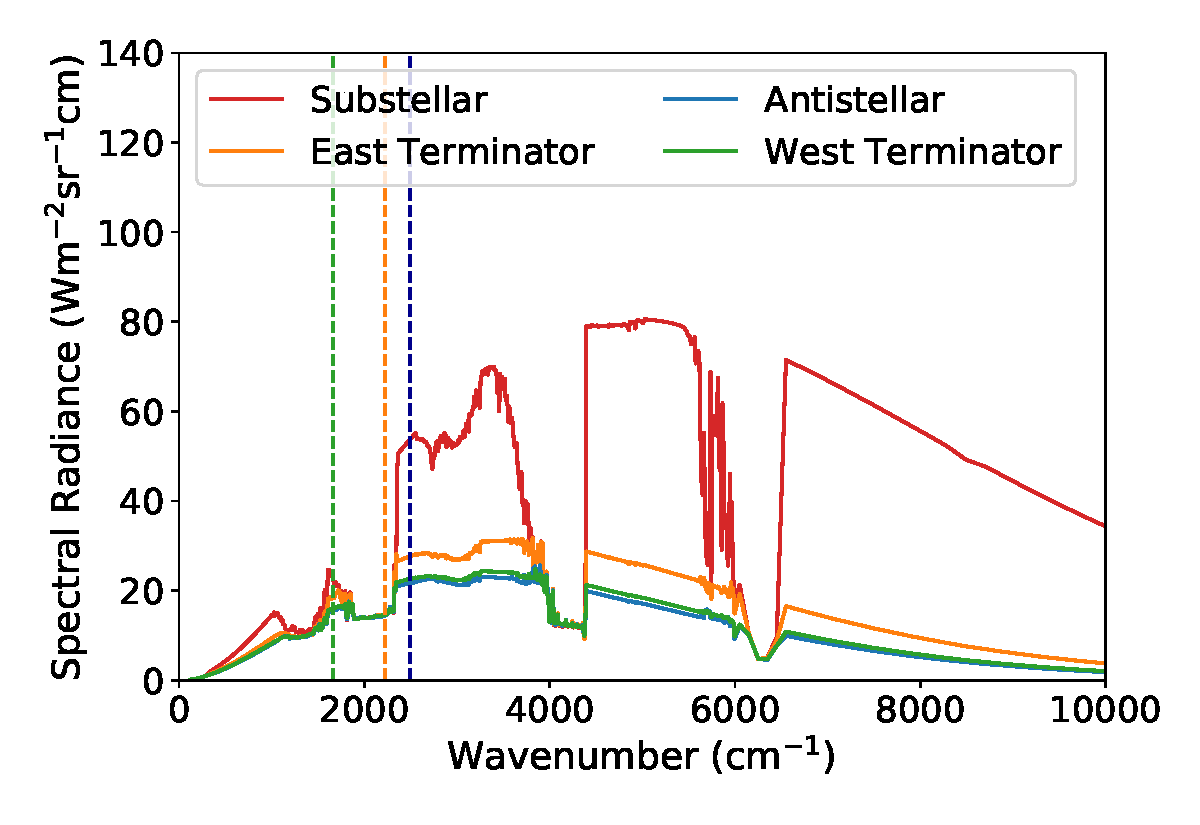
\includegraphics[width=\textwidth]{figures/soc-lava-planets/h2n2-spec-olr.pdf}
    \caption{Test 3: 10 bar mixed H$_{2}$-N$_{2}$ atmosphere.}\label{fig:soc-spec-olr-h2n2}
  \end{subfigure}
  %
  \begin{subfigure}[t]{0.49\textwidth}
    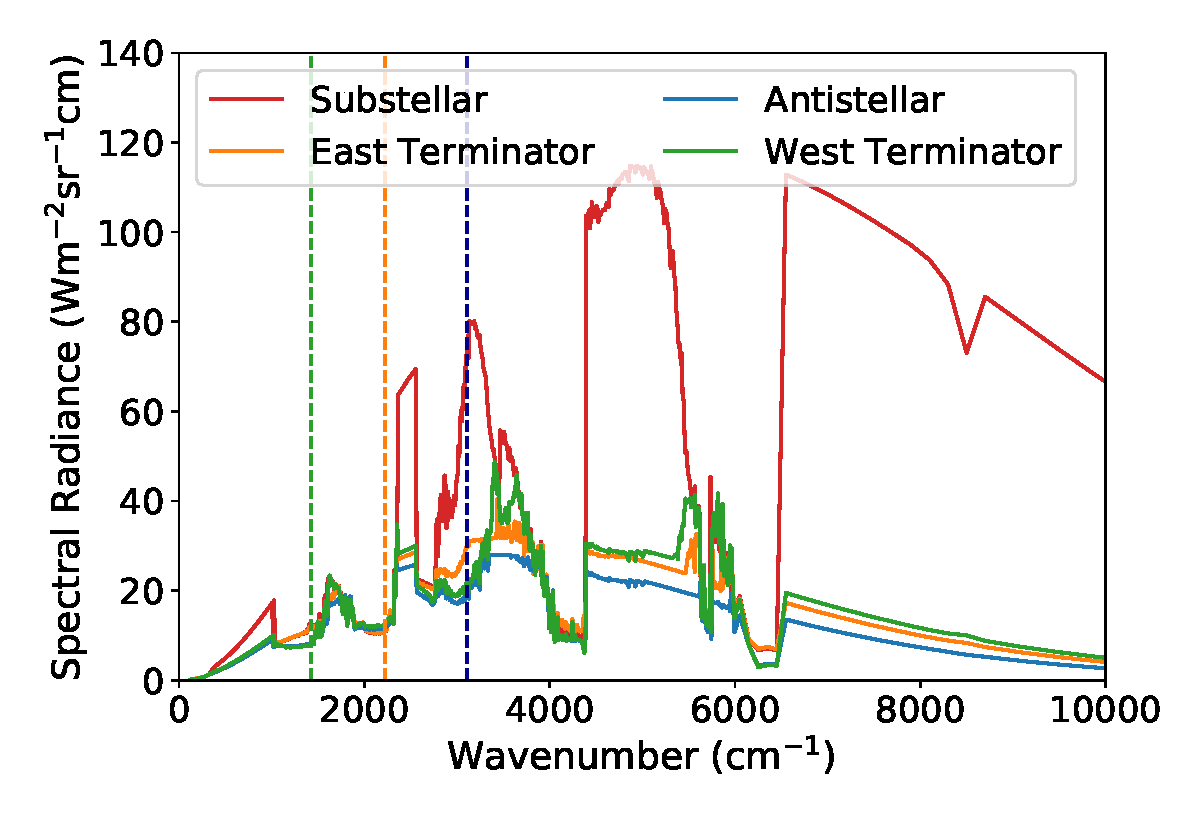
\includegraphics[width=\textwidth]{figures/soc-lava-planets/n2-100bar-spec-olr.pdf}
    \caption{Test 4: 100 bar N$_{2}$ atmosphere.}\label{fig:soc-spec-olr-n2-100bar}
  \end{subfigure}
  \caption{Outgoing longwave radiation of Tests 3 and 4 from various columns on their equators, showing the same CO absorption features as Figure \ref{fig:soc-spec-olr}.}
  \label{fig:soc-olr-best}
\end{figure}

\subsection{Thermal Emission}

Figure \ref{fig:soc-spec-olr-h2n2} shows the outgoing longwave radiation from atmospheric columns spaced evenly around the equator of Test 3. The CO absorption features have a greater magnitude than Test 1, but are small than those in Test 2. Figure \ref{fig:soc-emission-spec-h2n2} shows the emission spectra of the day-side and night-side of Test 3. The intermediate molecular weight of the atmosphere means that the heat redistribution is stronger than Test 2, but weaker than Test 1. This means that the magnitudes of the day-side and night-side spectra are closer than they are in Test 2, but are further apart than in Test 1. Observations of spectrally resolved phase curves could be compared to simulations like these to constrain the day-side and night-side temperature structures.


\begin{figure}
  \centering
  \begin{subfigure}[t]{0.49\textwidth}
    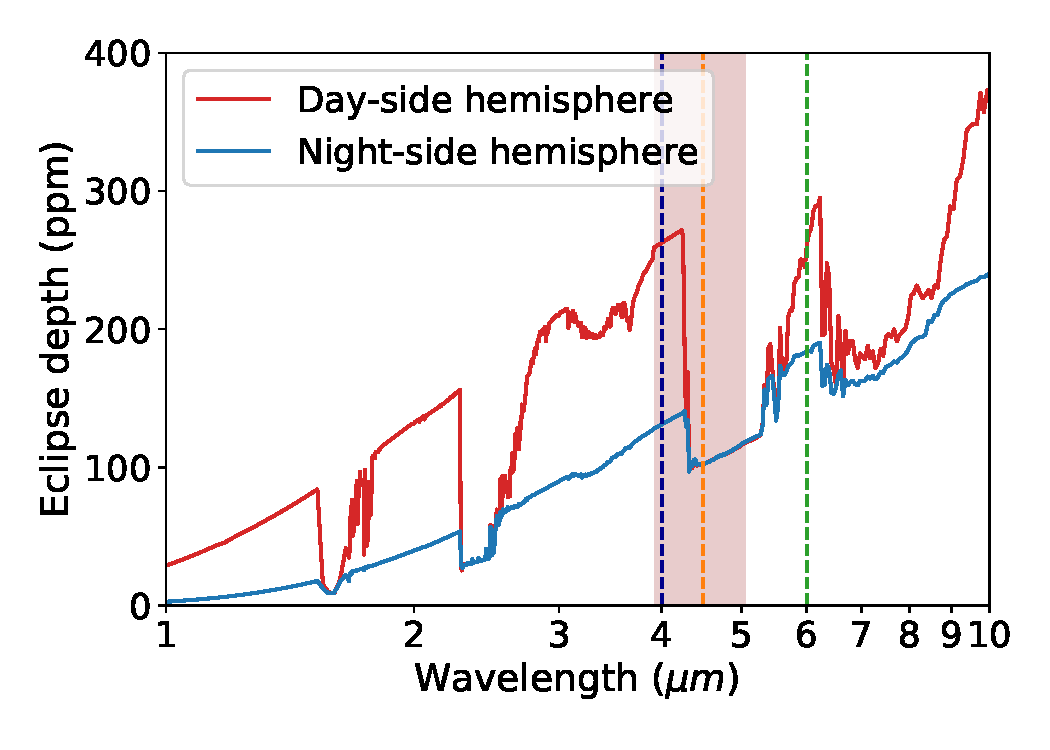
\includegraphics[width=\textwidth]{figures/soc-lava-planets/h2n2-emission-spec.pdf}
    \caption{Test 3: 10 bar mixed H$_{2}$-N$_{2}$ atmosphere.}\label{fig:soc-emission-spec-h2n2}
  \end{subfigure}
  %
  \begin{subfigure}[t]{0.49\textwidth}
    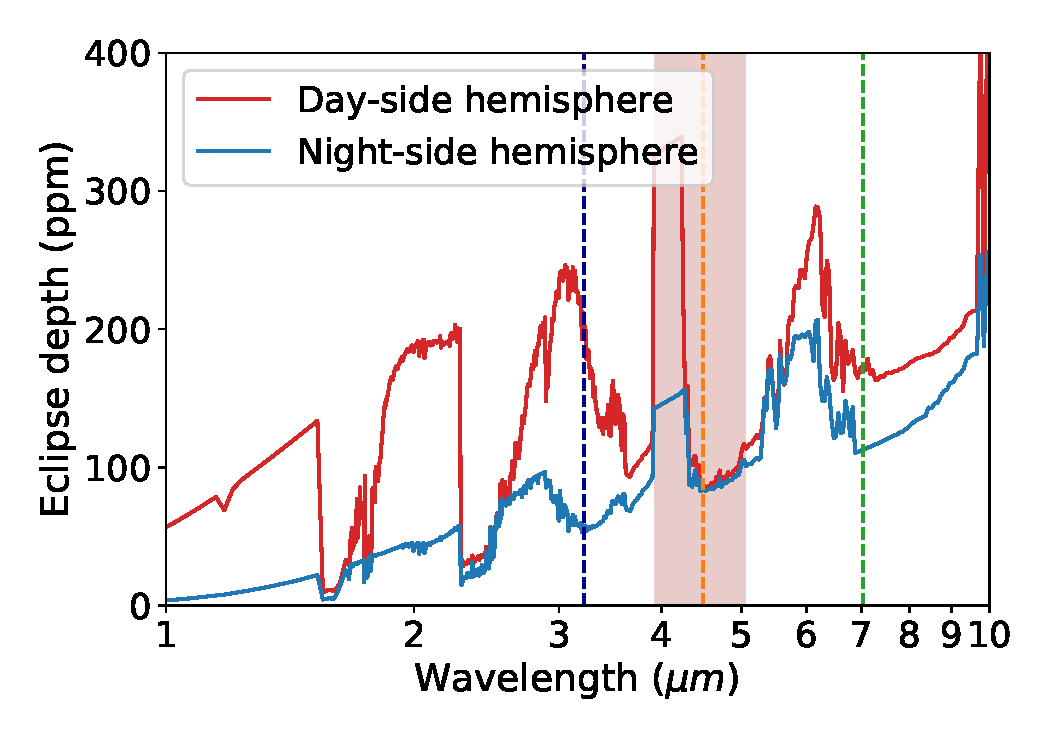
\includegraphics[width=\textwidth]{figures/soc-lava-planets/n2-100bar-emission-spec.pdf}
    \caption{Test 4: 100 bar N$_{2}$ atmosphere.}\label{fig:soc-emission-spec-n2-100bar}
  \end{subfigure}
  \caption{Thermal emission spectra of the day-sides and night-sides of Tests 3 and 4, showing the same absorption features as Figure \ref{fig:soc-olr-best} and relative magnitudes that depend on the atmospheric heat distribution efficiency.}
  \label{fig:soc-emission-spec-best}
\end{figure}

% (PLOT OLR MAP - SHOW NO HOT-SPOT SHIFT?)


% \begin{figure}
%   \centering
%     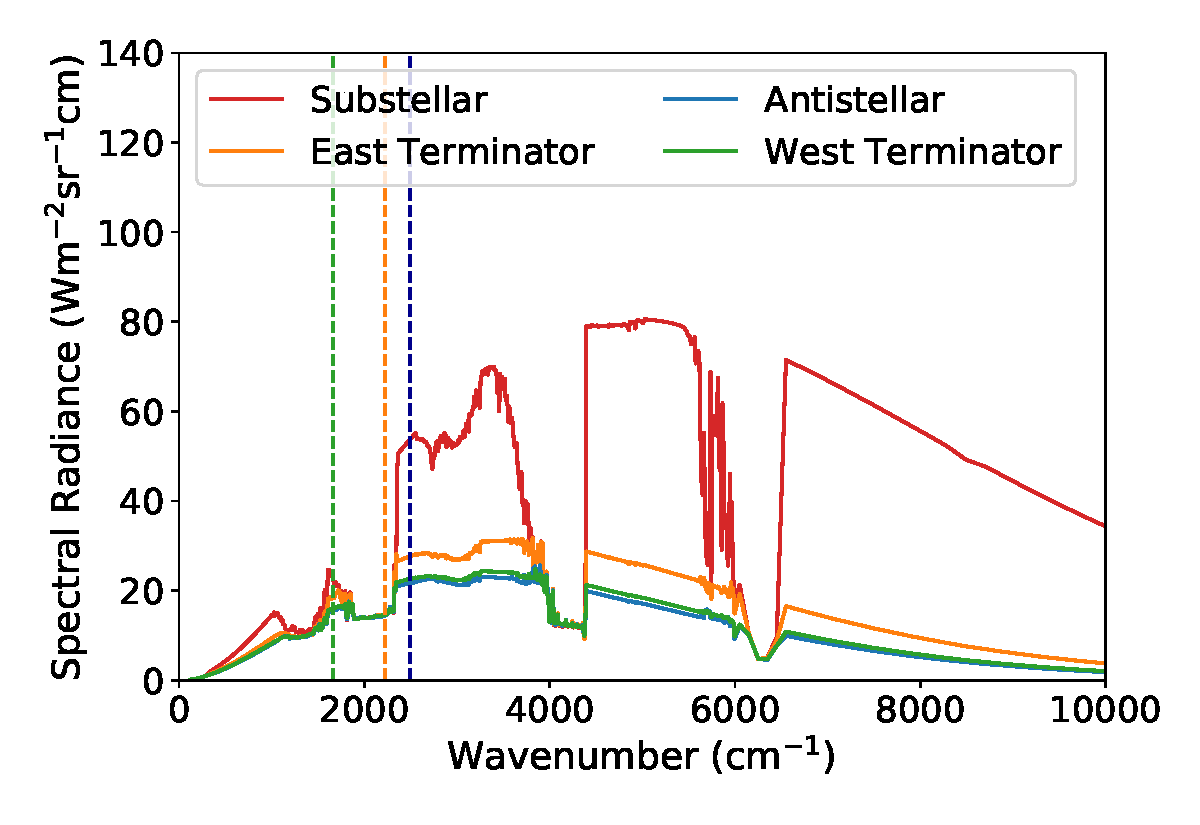
\includegraphics[width=0.49\textwidth]{figures/soc-lava-planets/h2n2-spec-olr.pdf}
%     \caption{10 bar mixed H$_{2}$-N$_{2}$ atmosphere.}\label{fig:soc-tp-h2n2}
% \end{figure}


% \begin{figure}
%   \centering
%     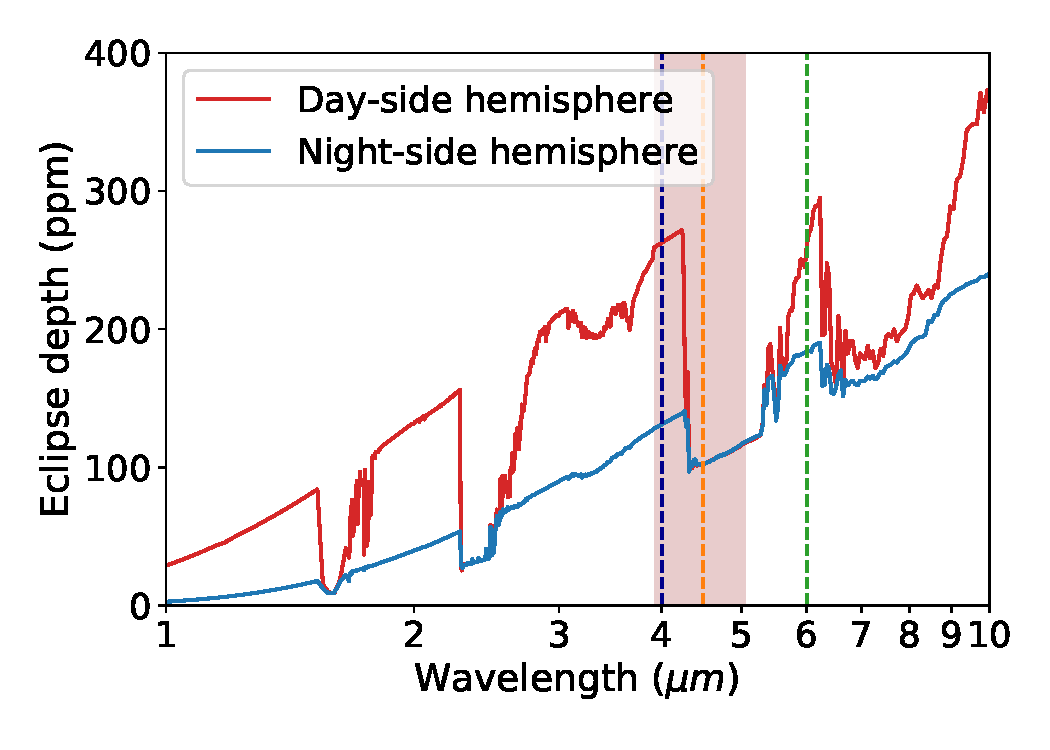
\includegraphics[width=0.49\textwidth]{figures/soc-lava-planets/h2n2-emission-spec.pdf}
%     \caption{10 bar mixed H$_{2}$-N$_{2}$ atmosphere.}\label{fig:soc-tp-h2n2}
% \end{figure}

\subsection{Thermal Phase Curves}

Figure \ref{fig:soc-spec-pc-h2n2} shows phase curves simulated from the thermal emission of Test 3, in the same spectral bands as Figure \ref{fig:soc-spec-pc}. The best-fit test in Chapter \ref{ch:linking-climate-55cnce} produced a phase curve that matched the hot-spot shift observed by \citet{demory201655cnce}. However, Test 3 does not have a phase offset in any of its phase curves, despite the hot-spot shift in its temperature field.

The \textit{Spitzer} bandpass and the wavelengths chosen for the phase curves cover a range of atmospheric opacities, so should probe a range of radiating levels. The phase curves at low and high atmospheric opacities have large and small amplitudes respectively, as discussed previously for the control test. The phase curves at the intermediate opacity of \SI{6.0}{\micro\metre} and in the \textit{Spitzer} band should probe the mid-atmosphere where the hot-spot shift is present. They show no phase shift, unlike the equivalent test in the previous chapter.


% The corresponding test in the previous chapter produced the best-fitting phase curve to the observations of \citet{demory201655cnce}. However, the phase curves of Test 3 in Figure \ref{fig:soc-spec-pc} show no significant hot-spot shift despite the large hot-spot shift in the temperature field in Figure \ref{fig:soc-temp-h2n2}.
%
% The wavelengths of the phase curves cover a range of opacities so should cover a range of radiating levels. As expected, the phase curves corresponding to low atmospheric opacity have a large amplitude (day-night contrast) as they are dominated by emission from the surface. At higher opacities, the thermal emission is higher in the atmosphere so the phase curve amplitude is smaller. But there is no phase offset for the phase curve at intermediate opacity as might be expected.


So, why does the hot-spot shift in the temperature field not appear in these phase curves? The hot-spot shift is not as large as the equivalent test in the previous chapter, but should still be large enough to shift the position of the maximum thermal emission at the level of the jet. However, the thermal emission from the surface appears to dominate the emission from the pressure level of the jet at the wavelength plotted (apart from \SI{4.5}{\micro\metre}, where the phase curve is from high in the atmosphere and is almost flat). The surface temperature is closely coupled to the incoming stellar radiation, so has no hot-spot shift. This shows that the atmosphere is too thin to observe the hot-spot shift in the temperature field, as the surface dominates the thermal emission. Hot-spot shifts are regularly observed and simulated in the atmospheres of hot Jupiters \citep{zellem2014hd209, showman2015circulation}, suggesting that a sufficiently thick atmosphere is required for a phase offset in the outgoing longwave radiation. The next section will show the results of a simulation of a 100 bar atmosphere on 55 Cancri e, which will be thick enough to produce an observable offset in its thermal phase curve.

 % On hot Jupiters, the hot-spot shift is visible in thermal phase curves as the jet often extends over a wide range of pressure levels and there is no significantly hotter surface to dominate the emission. I will discuss this in more detail in Section \ref{sec:soc-lava-discussion}.
%
% For now, I will suggest the hypothesis that it is not possible to observe a hot-spot shift on a tidally locked planet without a sufficiently thick atmosphere. In the next section I will test a 100 bar atmosphere on 55 Cancri e to determine if the hot-spot shift appears in its thermal phase curve.

\begin{figure}
  \centering
  \begin{subfigure}[t]{0.48\textwidth}
    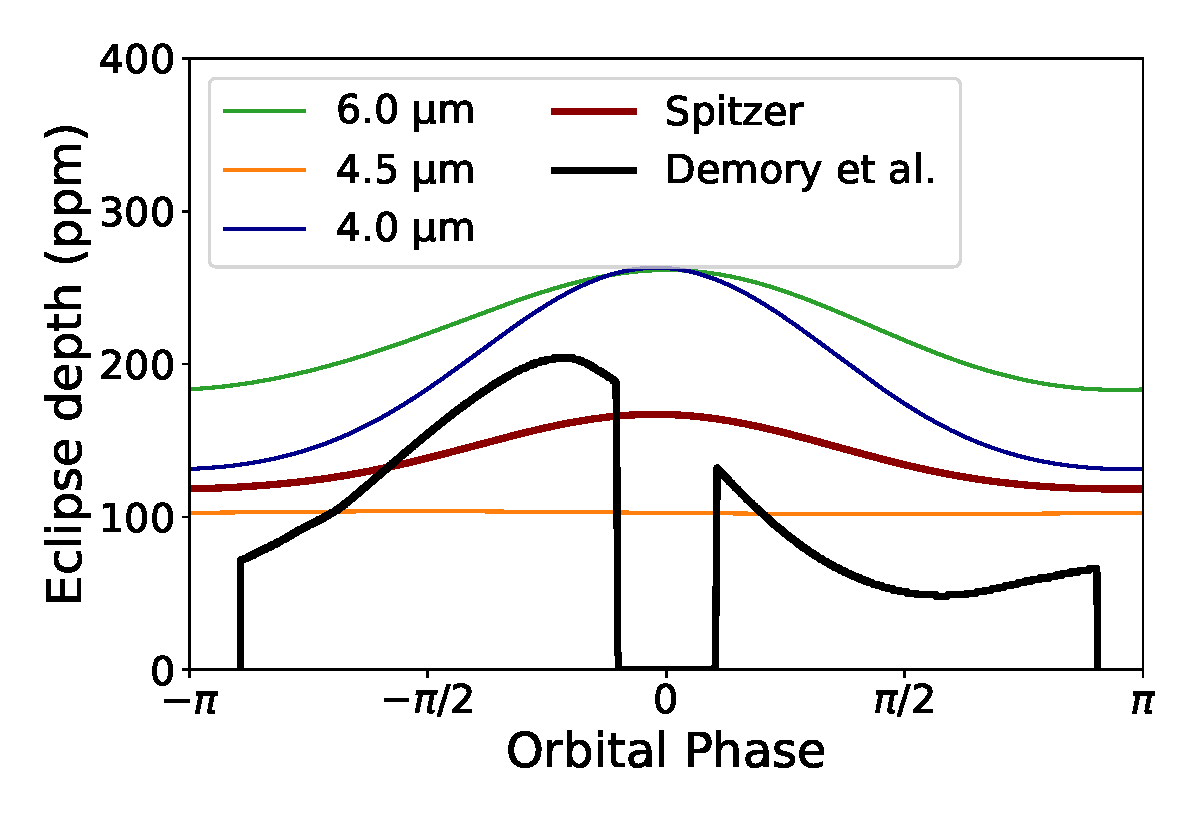
\includegraphics[width=\textwidth]{figures/soc-lava-planets/h2n2-spec-pc.pdf}
    \caption{Test 3: 10 bar mixed H$_{2}$-N$_{2}$ atmosphere.}\label{fig:soc-spec-pc-h2n2}
  \end{subfigure}
\quad
  \begin{subfigure}[t]{0.48\textwidth}
    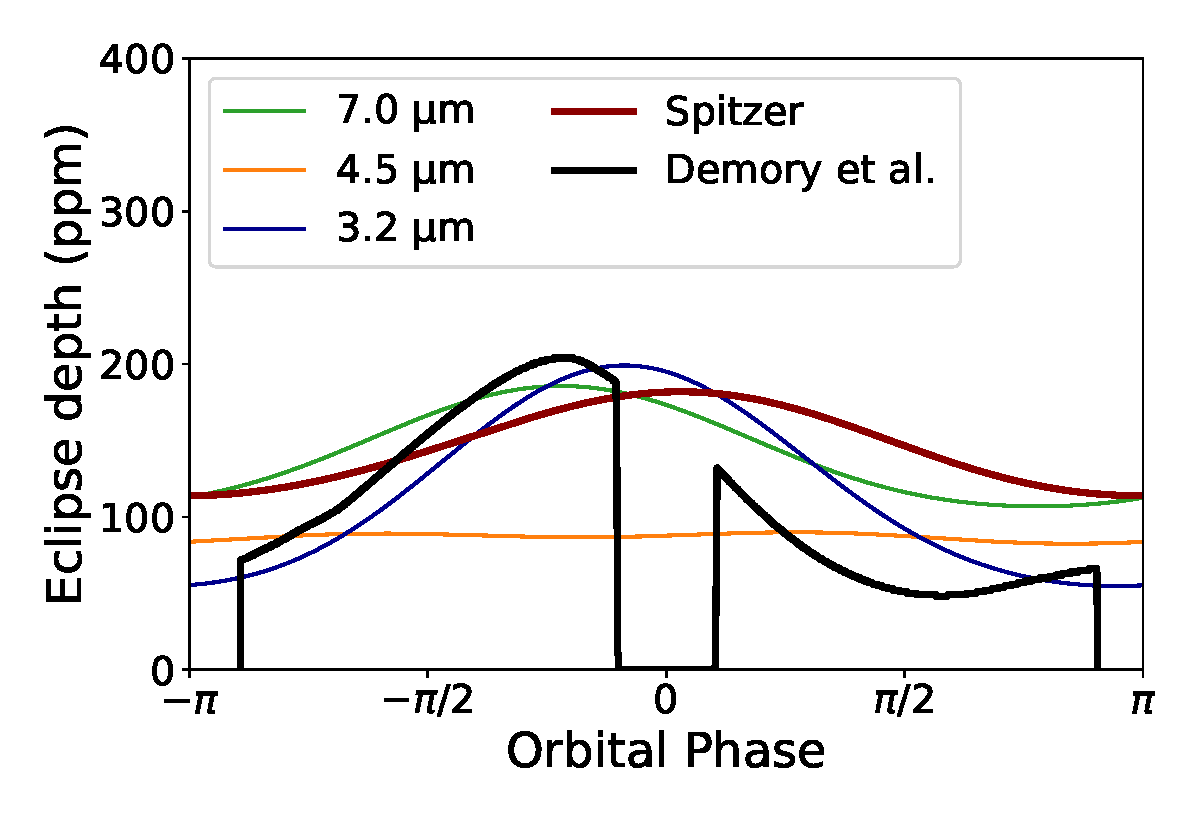
\includegraphics[width=\textwidth]{figures/soc-lava-planets/n2-100bar-spec-pc.pdf}
    \caption{Test 4: 100 bar N$_{2}$ atmosphere.}\label{fig:soc-spec-pc-n2-100bar}
  \end{subfigure}
  \caption{Phase curves at different wavelengths and in the \textit{Spitzer} bandpass of Tests 3 and 4. Test 3 has no phase offset at any wavelength, due to its thin atmosphere. Test 4 has a significant phase offset at \SI{7.0}{\micro\metre}, due to its thick atmosphere.}
  \label{fig:soc-spec-pc-best}
\end{figure}


% \begin{figure}
%   \centering
%     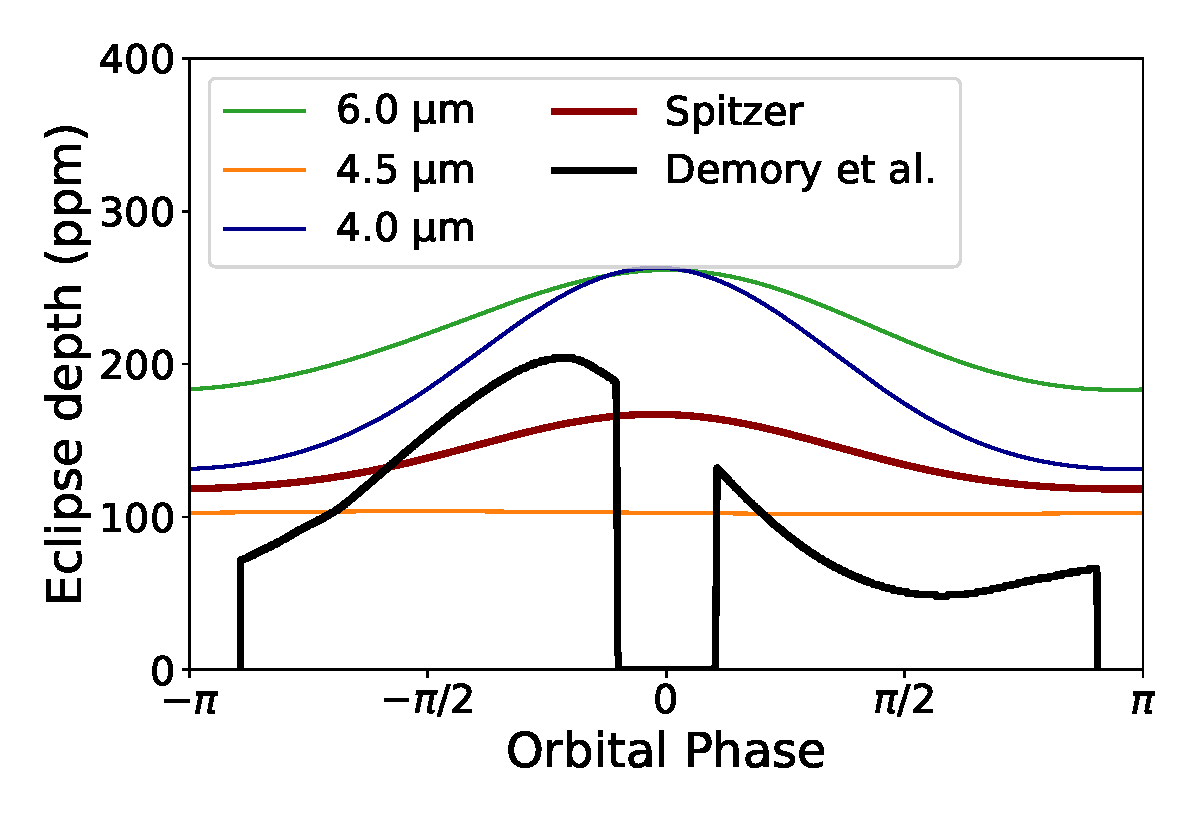
\includegraphics[width=0.49\textwidth]{figures/soc-lava-planets/h2n2-spec-pc.pdf}
%     \caption{10 bar H$_{2}$ atmosphere.}\label{fig:soc-spec-pc-h2n2}
% \end{figure}

% \subsection{Contribution Function}\label{sec:contrib-func-h2n2}
%
% The contribution function shows that the surface dominates
%
% Figure X shows the contribution function at \SI{4.0}{\micro\metre}, where the atmospheric opacity is low. The contribution function is dominated by the surface. This is why the phase curve in Figure X is X.
%
% Figure X shows the contribution function at \SI{4.0}{\micro\metre}, where the atmospheric opacity is high. The contribution function is dominated by the upper atmosphere. This is why the phase curve in Figure X is X.
%
% It appears difficult to observe a phase curve at a wavelength that shows the hot-spot shift that is apparent in the temperature field for this atmosphere. If the opacity is such that significant flux comes from the jet level, there is always more flux dominating it from the surface. I will discuss this in more detail later.


%%%%%%%%%%%%%%%%%%%%%%%%%%%%%%%%%%%%
\section{Thick Atmosphere Results}\label{sec:100-bar-simulation}

This section shows the results of Test 4, a simulation with a 100 bar surface pressure, to test the hypothesis that a sufficiently thick atmosphere is required for an offset in the thermal phase curve. The higher mean molecular weight of its N$_{2}$ atmosphere balances the effect of the increased surface pressure, which would otherwise increase the radiative timescale and decrease the hot-spot shift.

Significant emission from the pressure level of the equatorial jet is needed for an offset in the thermal phase curve, so that emission from the hot-spot shift dominates emission from the level heated in phase with the stellar radiation. In the 10 bar atmospheres earlier, the thermal emission was always dominated by emission from the surface which has no hot-spot shift. At wavelengths where the atmospheric opacity was high, such as the \SI{4.5}{\micro\metre} phase curves earlier, the emission from the jet level dominated the emission from the surface. However, the high opacity meant that the phase curve reflected a radiating level high in the atmosphere so was almost flat.

This section will show that there is an observable hot-spot shift in the temperature field and outgoing longwave radiation of Test 4, supporting the hypothesis that a thick atmosphere is needed to observe a hot-spot shift. This thick atmosphere is more similar to a hot Jupiter, where hot-spot shifts are commonly simulated and observed. I will conclude that this simulation is evidence for an atmosphere on 55 Cancri e with a surface pressure greater than 10 bar.


%
% The  main question arising from the simulations so far is how such a large hot-spot shift was observed by \citet{demory201655cnce}, given the difficulty in recreating it from the simulated OLR. Test 3 has a hot-spot shift of up to \ang{90} on the equator and seems well suited to show this in its thermal emission. However, the OLR is either dominated by at low opacities by the surface emission with no hot-spot shift, or at high opacities by the top-of-atmosphere emission.

% For an atmosphere of 10 bar, a very specific opacity is required to observed the hot-spot shift, which is only significant in the relatively small pressure range containing the equatorial jet (as shown in the earlier plots of the zonal-mean zonal wind). It seems unlikely that the whole bandpass of the observed phase curve (from about $4$ to \SI{5}{\micro\metre}) would have an opacity exactly right for this.

% What could produce an atmosphere with an observable hot-spot shift? The equatorial jet and hot-spot shift forms above the level of the thermal forcing. Therefore, the radiating level must correspond to the level of the hot-spot shift, with minimal contribution from the level of the thermal forcing. The main problem for these 10 bar atmospheres is that the outgoing radiation is always dominated by the thermal emission of the surface unless the opacity at the observed wavelength is very high. For very high opacity, the emission from the hot-spot shift may be very weak or be dominated by emission from the upper atmosphere.

% The shortwave radiation therefore needs to be absorbed over a larger range, at higher pressures than the level of the jet. Then, the outgoing radiation at a moderate opacity will represent the hot-spot shift at the level of the jet, without being dominated by a surface emitting close below.

% So an observable shift requires a thicker atmosphere, with more longwave optical depth between the level of shortwave heating and the level of the jet. This is more like the atmosphere of a hot Jupiter, where the jet is produced by shortwave heating of a range of levels, and the temperature increases less rapidly with depth than in the convective layer of the terrestrial atmospheres of this chapter. Hot Jupiters do indeed display hot-spot shifts in their observed and simulated phase curves \citep{amundsen2016hd209}.

% In this section, I therefore show the results of Test 4, a 100 bar N$_{2}$ atmosphere with otherwise the same parameters as the previous tests. The increased surface pressure should give a longer radiative timescale, increasing the expected hot-spot shift compared to the 10 bar Test 2. I will discuss the global circulation and the simulated observations, and will show that a hot-spot shift is now apparent in the thermal phase curve at some wavelengths.


\subsection{Global Circulation}

 Figure \ref{fig:soc-temp-n2-100bar} shows the global temperature map and winds at the pressure level of Test 4 where the equatorial jet is strongest,  as a time-average from 200 to 400 days. There is a strong eastward hot-spot shift and a large day-night contrast. Test 2 had a similar 10 bar N$_{2}$ atmosphere with no hot-spot shift in Figure \ref{fig:soc-temp}; the hot-spot shift in Test 4 is due to the increased radiative timescale caused by the higher surface pressure \citep{zhang2017dynamics}.

Figure \ref{fig:soc-zonal-u-n2-100bar} shows the zonal-mean zonal wind of Test 4. It is similar to the zonal wind of a hot Jupiter simulation, where the equatorial jet extends through many pressure levels due to shortwave heating through the atmosphere \citep{showman2015circulation}. The prograde eastward flow at all latitudes at the level of the maximum equatorial jet speed is explained by the mechanism discussed in Chapter \ref{ch:eqm-zonal-flow}.

Figure \ref{fig:soc-tp-n2-100bar} shows the temperature profiles around the equator of this test. They are similar to the temperature profiles of the other tests, but show higher temperatures high on the day-side due to the increased effect of shortwave absorption. In reality, a 100 bar atmosphere would have a higher opacity at all wavelengths due to collision-induced absorption, so shortwave absorption would play a greater role in the temperature profiles, as in the atmospheres of hot Jupiters \citep{amundsen2016hd209}.



%
% \begin{figure}
%   \centering
%     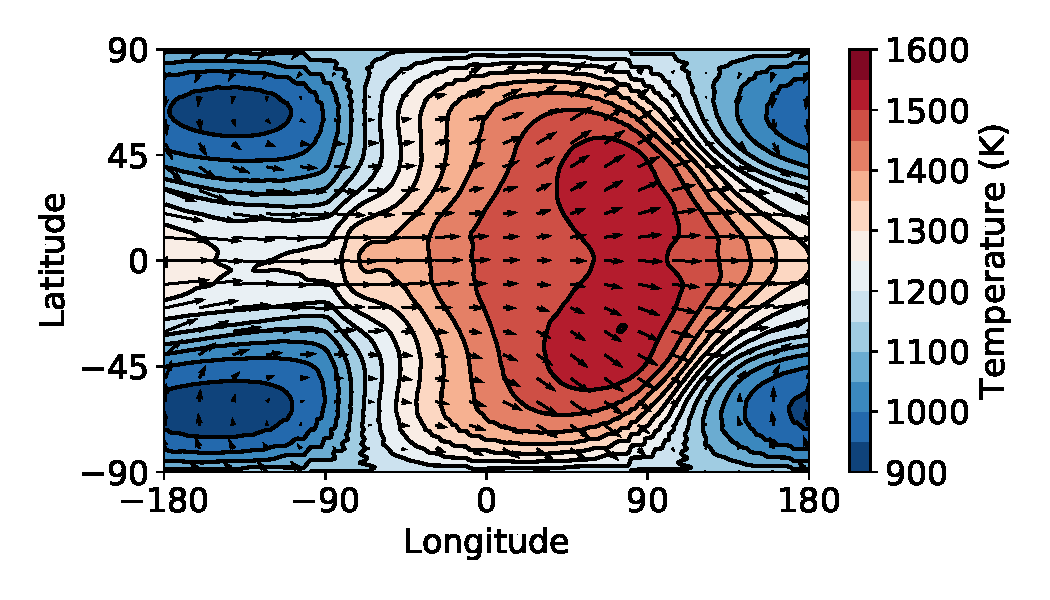
\includegraphics[width=0.49\textwidth]{figures/soc-lava-planets/n2-100bar-soc-temp.pdf}
%     \caption{Global temperature maps of the 100 bar N$_{2}$ test at the X pressure level.}\label{fig:soc-temp-n2-100bar}
% \end{figure}
%
%
% \begin{figure}
%   \centering
%     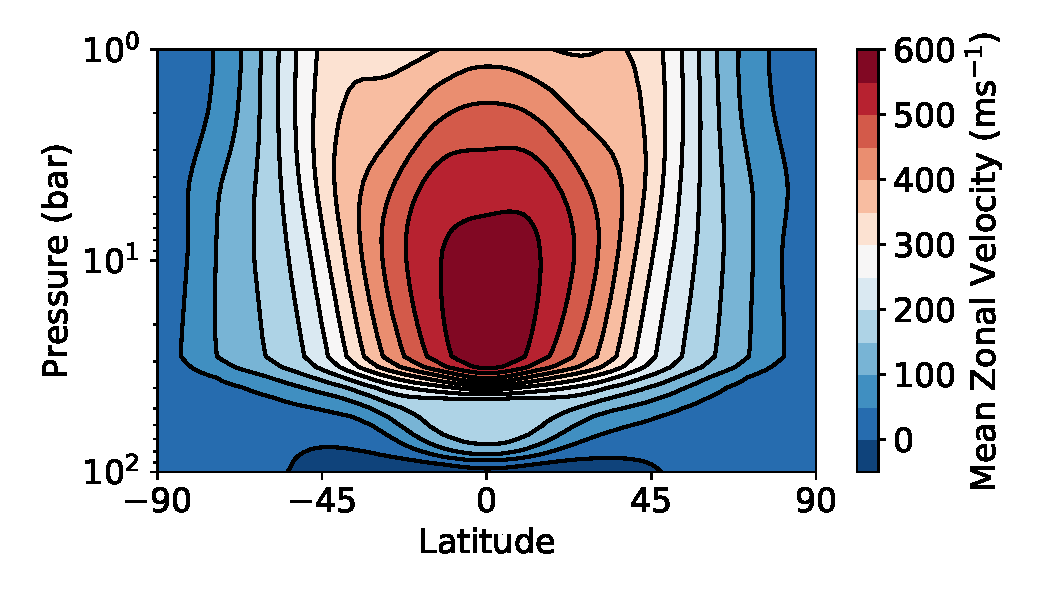
\includegraphics[width=0.49\textwidth]{figures/soc-lava-planets/n2-100bar-soc-zonal-u.pdf}
%     \caption{Zonal-mean zonal wind of the 100 bar N$_{2}$ test.}\label{fig:soc-zonal-u-n2-100bar}
% \end{figure}
%
%
% \begin{figure}
%   \centering
%     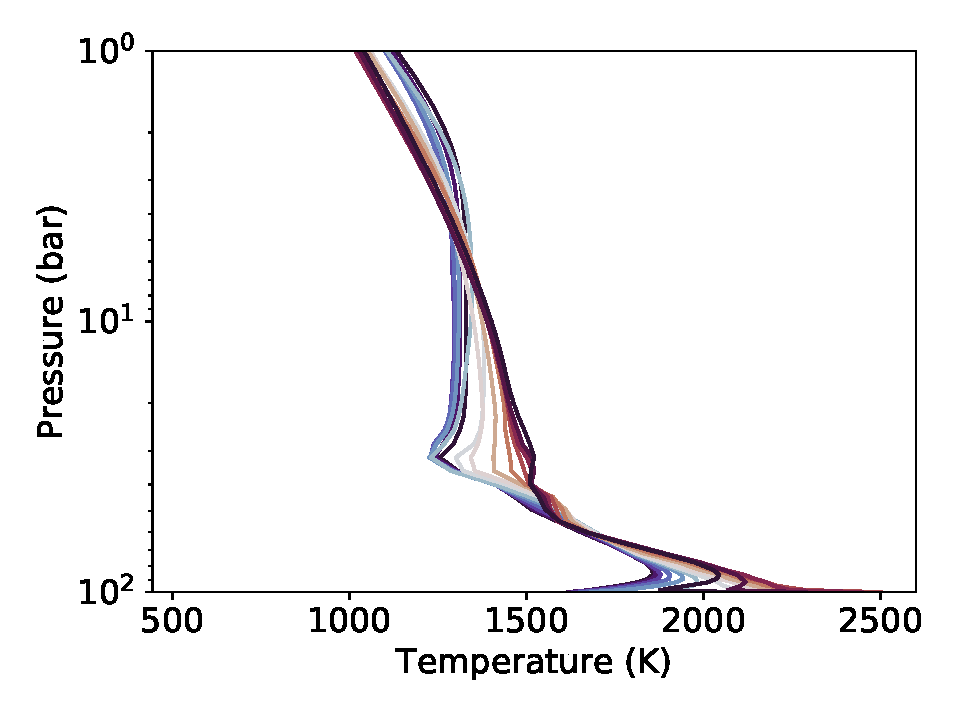
\includegraphics[width=0.49\textwidth]{figures/soc-lava-planets/n2-100bar-soc-tp.pdf}
%     \caption{Temperature profiles of the 100 bar N$_{2}$ test.}\label{fig:soc-tp-n2-100bar}
% \end{figure}



\subsection{Thermal Emission}

Figure \ref{fig:soc-spec-olr-n2-100bar} shows the outgoing longwave radiation from the substellar point, antistellar point, and terminators on the equator of Test 4. The spectrum has the same absorption features as before, with deeper features than the other tests in regions of intermediate opacity due to the thicker atmosphere. Figure \ref{fig:soc-emission-spec-n2-100bar} shows the emission spectrum of the day-side and night-side of Test 4, which also has deeper absorption features than the previous tests.  The magnitude of the emission is higher than the previous tests, due to the increased surface temperature of the thicker atmosphere. As discussed above,  in reality such a thick atmosphere would have a higher opacity in the absorption windows in this test, meaning that the emission from the surface would not appear in the OLR. However, this idealised situation is useful for comparing the effect of different opacities on the thermal emission and phase curves.



% \begin{figure}
%   \centering
%     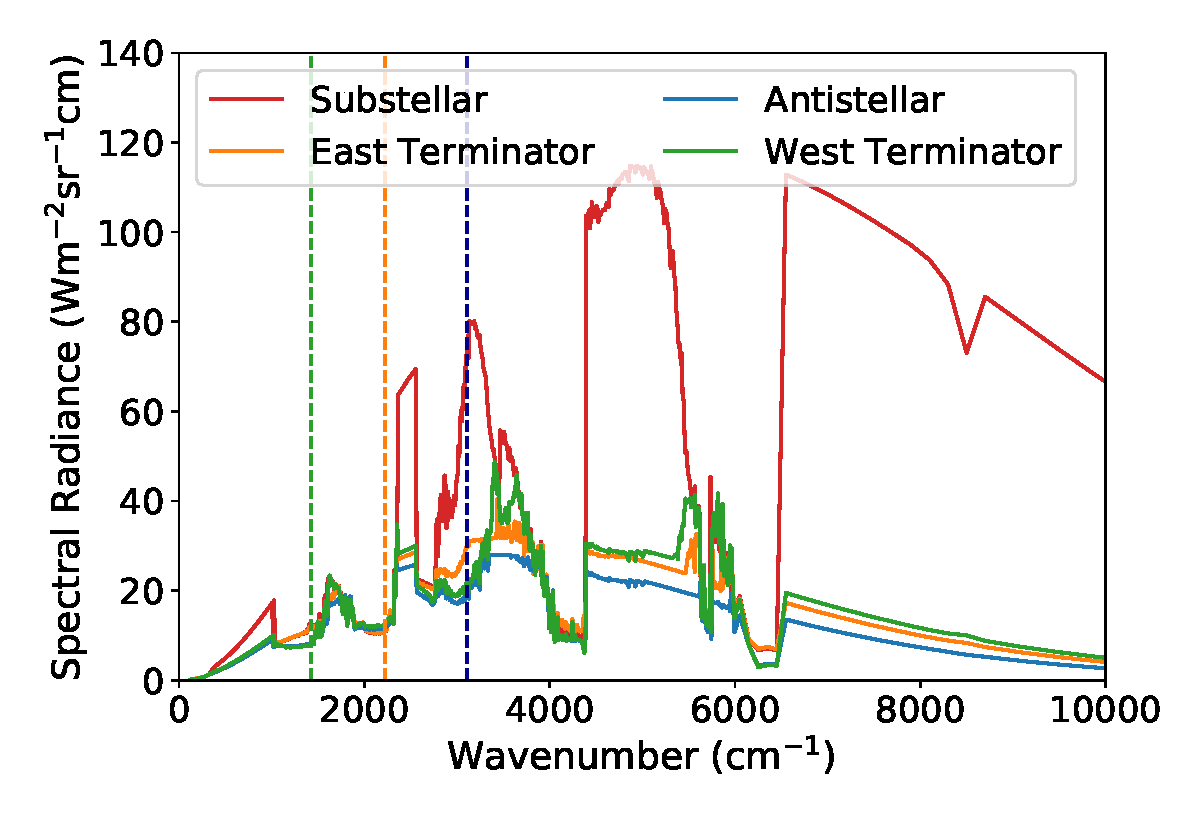
\includegraphics[width=0.49\textwidth]{figures/soc-lava-planets/n2-100bar-spec-olr.pdf}
%     \caption{100 bar N$_{2}$ atmosphere.}\label{fig:soc-tp-n2-100bar}
% \end{figure}


% \begin{figure}
%   \centering
%     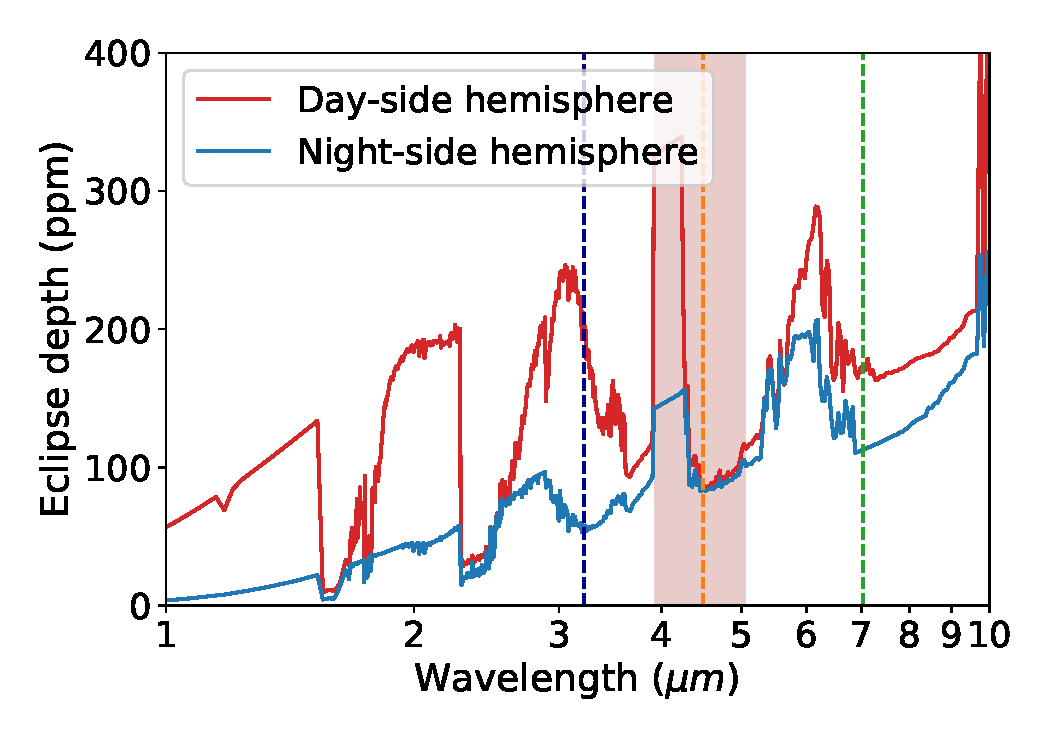
\includegraphics[width=0.49\textwidth]{figures/soc-lava-planets/n2-100bar-emission-spec.pdf}
%     \caption{100 bar N$_{2}$ atmosphere.}\label{fig:soc-tp-n2-100bar}
% \end{figure}

\subsection{Thermal Phase Curves}

Figure \ref{fig:soc-spec-pc-n2-100bar} shows phase curves calculated from Test 4 at various wavelengths and in the \textit{Spitzer} \SI{4.5}{\micro\metre} bandpass. Note that the wavelengths of the phase curves are different to those chosen for the previous tests, to highlight new behaviour. The green phase curve at \SI{7.0}{\micro\metre} has a large phase offset, a feature that did not appear in the phase curves of the other tests in this chapter. This supports the hypothesis that a sufficiently thick atmosphere is required to observe a hot-spot shift in the phase curve. The blue \SI{3.2}{\micro\metre} phase curve matches the day-side and night-side temperature of the observed phase curve, but not the hot-spot shift. The \SI{4.5}{\micro\metre} opacity is very high, so the phase curve at that wavelength has almost zero amplitude. Even if there were a hot-spot shift at this wavelength it would not be visible due to the small amplitude of the phase curve.

The thick red line calculated in the \textit{Spitzer} bandpass does not match the observations. This suggests that the CO-dominated radiative transfer in the simulations is not a good model of the observed atmosphere. This is not a problem for the conclusions of this chapter, which seeks to show the general effect of variable atmospheric opacity on the global circulation and observed thermal emission. It would be possible to tune the atmospheric radiative properties to probe exactly the right level in the \textit{Spitzer} bandpass, but this would be an artificial fit without any observational constraints of composition. More observations such as emission spectra are needed to constrain the composition, which would allow for further modelling with more accurate parameters.

I therefore suggest that the observation of the hot-spot shift on 55 Cancri e is evidence for an atmosphere with a higher surface pressure than 10 bar. This is a different conclusion to Chapter \ref{ch:linking-climate-55cnce}, which suggested an atmosphere of 1 to 10 bar produced the maximum hot-spot shift. Chapter \ref{ch:linking-climate-55cnce} aimed to find the maximum hot-spot shift and day-night contrast in the temperature field only. This chapter has sought to find the maximum phase offset and amplitude in the thermal phase curve from the spectrally resolved outgoing longwave radiation, which also requires a sufficiently thick atmosphere. So, the conclusions of the chapters are different but do not contradict each other.
 %
 %
 % This is not inconsistent with the results of Chapter \ref{ch:linking-climate-55cnce}, where the scaling relations and GCM simulations suggested a maximum hot-spot shift and a best-fit atmosphere of around 10 bar. This was true -- the physical hot-spot shift in temperature does benefit from an atmosphere that is not too thick. The key point is that this hot-spot shift will not show up in the outgoing thermal radiation for a 10 bar atmosphere, and so a thicker atmosphere is required.

% \begin{figure}
%   \centering
%     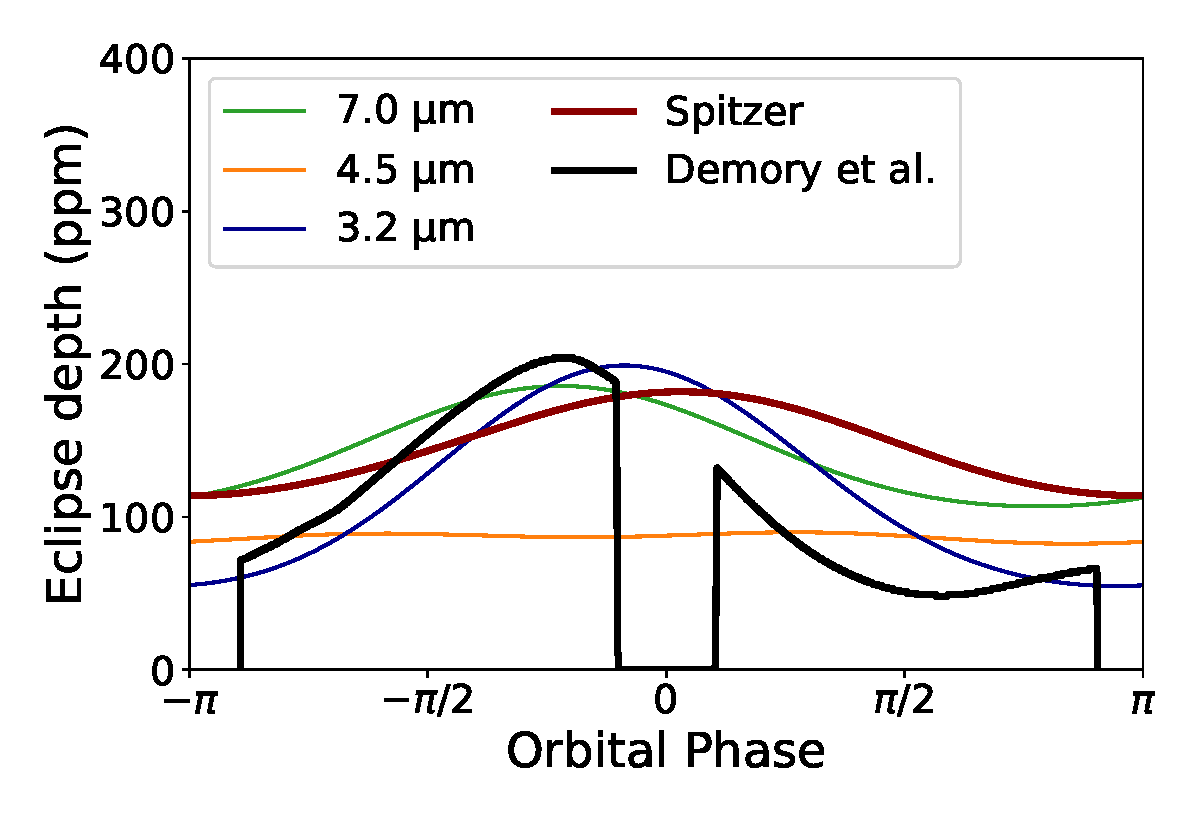
\includegraphics[width=0.49\textwidth]{figures/soc-lava-planets/n2-100bar-spec-pc.pdf}
%     \caption{100 bar N$_{2}$ atmosphere.}\label{fig:soc-spec-pc-n2-100bar}
% \end{figure}

% \subsection{Contribution Function}\label{sec:contrib-func-100bar}
%
% Plot cont functions.



%%%%%%%%%%%%%%%%%%%%%%%%%%%%%%%%%%%%
\section{Discussion}\label{sec:soc-lava-discussion}


The first aim of this chapter was to compare the simulations using the new \textit{Socrates} radiative transfer scheme to the results of the semi-grey scheme in the previous chapter. Tests 1, 2, and 3 qualitatively matched the corresponding tests with the semi-grey model, showing that the scaling relations for hot-spot shift and day-night contrast apply to this more realistic model as well \citep{zhang2017dynamics}.

However, there was an important difference between the simulated thermal phase curves in this chapter and Chapter \ref{ch:linking-climate-55cnce}. Previously, the phase curves were calculated from the \SI{4.5}{\micro\metre} flux emitted from a particular atmospheric pressure level radiating as a black body. This approximation meant that if a hot-spot shift appeared in the temperature field at a particular pressure level, it had to appear in the thermal phase curve calculated using that level. The thermal phase curves in this chapter are instead calculated with the OLR simulated by the \textit{Socrates} radiative transfer scheme, which does not correspond to a single pressure level for a given wavelength. In Tests 1, 2, and 3 this meant that the emission from the surface dominated the emission from the relatively thin atmosphere at most wavelengths, reducing the effect of the atmospheric circulation on the phase curve. In particular, there was no phase offset in any of the phase curves calculated from Tests 1, 2, and 3.

This is due to the fact that surface temperature is higher than the jet layer temperature. The relative emission can be estimated with a simple model. If the lower atmosphere follows a dry adiabat and the jet layer is at half the surface pressure, the temperature of the jet layer is $T_{jet} = 0.5^{R/c_{p}}T_{surf}$, where $R/c_{p}$ is the dry adiabatic lapse rate. This gives $T_{jet} \approx 0.8 T_{surf}$ for an N$_{2}$ atmosphere, which means that the black-body emission from the surface is stronger than the emission from the level of the jet -- $B_{surf} \approx 2.4 B_{jet}$. Therefore, a sufficiently high opacity is required for the emission from the level of the jet to be stronger than the emission from the surface. However, this high opacity may mean that the emission from the jet is weakened, and the outgoing radiation is dominated by a level above the jet. There may be no appropriate opacity for a thin atmosphere to give a thermal phase curve dominated by emission from the level of the equatorial jet.





% In this chapter the thermal phase curves are instead calculated directly from the \textit{Socrates} radiative transfer scheme at specific wavelengths and in the \textit{Spitzer} \SI{4.5}{\micro\metre} bandpass. This means that a particular wavelength or band does not correspond to a single pressure level, and instead depends on the emission from the entire atmosphere. This is often dominated by a certain range of pressure levels, which is why the radiating level is a useful concept. However, in these tests the relatively low total surface pressure and the fact that the surface is always hotter than the atmosphere meant that the surface emission always dominated the emission of the level of the jet and hot-spot shift. This meant that a significant hot-spot shift did not appear in any of the phase curves of the tests with 10 bar surface pressure.


%%%%%%
%
% It is possible to explain this issue with a simple two-layer model of the surface and the pressure level of the hot-spot shift and jet.To observe the hot-spot shift, the flux from its level must be comparable to or greater than the flux from the surface. We assume that the jet forms one scale height above the surface, and assume that its temperature is $T_{jet} = e^{-1}T_{surf}$. Then if there is only one absorbing gas, the magnitudes of the OLR at a given wavelength $\lambda$ from the jet and the surface are \citep{pierrehumbert2010principles}:
%
% \begin{equation}
%   OLR_{surf} = B_{surf}(T_{surf},\lambda)  e^{-\kappa w \rho_{0} H},
% \end{equation}
%
% \begin{equation}
%   OLR_{jet} = B_{jet}(T_{jet},\lambda)  e^{-\kappa w \rho_{0} H e^{-1}},
% \end{equation}
%
% where $B(T,\lambda)$ is the Planck function, $\kappa$ is the opacity, $w$ is the mixing ratio of the absorber, $\rho_{0}$ is the density at the surface and $H$ is the scale height.
%
% For a low opacity $\kappa$, the flux from the surface will dominate, and vice versa. The opacity must therefore be sufficiently high for the flux from the jet to dominate the flux from the surface. However, if the opacity is too large then $e^{-\kappa w \rho_{0} H e^{-1}}$ is too small and there is too little OLR to observe anything (or, it will be dominated by emission from the upper atmosphere above the jet). A hot-spot shift is therefore not observable on a terrestrial planet if the minimum opacity for the OLR from the jet to dominate the OLR from the surface is so large that the jet OLR is then too small to observe.
%
% Setting the two fluxes equal gives the opacity at which they cross, and so the minimum opacity for the flux from the jet level to dominate:
%
% \begin{equation}
%   B_{surf}(T_{surf},\lambda)  e^{-\kappa_{min} w \rho_{0} H} = B_{jet}(T_{jet},\lambda)  e^{-\kappa_{min} w \rho_{0} H e^{-1}}
% \end{equation}
%
% \begin{equation}
%   \frac{T_{jet}^{4}}{T_{surf}^{4}} e^{-\kappa_{min}w\rho_{0}H(e^{-1}-1)} = 1
% \end{equation}
%
% As $T_{jet} = e^{-1}T_{surf}$,
%
% \begin{equation}
%   \kappa_{min} w = \frac{4 e}{\rho_{0} H}
% \end{equation}
%
% For a scale height $H=1\times 10^{4}\ \mathrm{m}$ and a surface density of $1\  \mathrm{kg m}^{-1}$, this gives a value of $\kappa_{min} w \approx 1\times 10^{-3}$. This means that the OLR from the jet level is attenuated from the original Planck function by $e^{-\kappa_{min} w \rho_{0} H e^{-1}} = e^{-4}$, or $1.83\%$ of the original value, making it all but unobservable in relation to the upper atmosphere or other effects. So, in this model system of a terrestrial planet with a relatively thin atmosphere dominated by longwave heating from the surface, there is no wavelength or opacity at which we can observe a hot-spot shift. It is either dominated by the surface at low opacities, or attenuated to less than $1.83\%$ when the opacity is high enough that the surface does not dominate.

Therefore, it is unlikely that a hot-spot shift will appear in the thermal phase curve of a terrestrial planet with a thin atmosphere. Hot-spot shifts are regularly seen in observations and simulations of hot Jupiters with thick atmospheres \citep{amundsen2016hd209, parmentier2017handbook}. Hot Jupiters have much deeper zonal jets due to the shortwave heating through a large range of pressure levels of their atmosphere, rather than the longwave heating that produces a strongly forced jet in a small pressure range on a terrestrial planet. They also have much thicker atmospheres, meaning that the thermal emission from the potentially hotter deep atmosphere does not affect the OLR, unlike the emission from the surface in these terrestrial planets.

 The results in this chapter suggest that a hot-spot shift will appear in the thermal emission only for a surface pressure of at least 10 to \SI{100}{\bar}. This effect accounts for the difference between the 10 bar tests and the 100 bar Test 4, where a hot-spot shift only appeared in the thermal phase curve of the thicker atmosphere. These simulations therefore present a different conclusion to those in Chapter \ref{ch:linking-climate-55cnce}. Instead of a 5 bar atmosphere with a mean-molecular weight of \SI{4.6}{\gram\per\mole}, they suggest that an atmosphere thicker than 10 bar is required, and that a heavier mean molecular weight may be required to compensate for the increased radiative timescale.

 This conclusion does not contradict the work in Chapter \ref{ch:linking-climate-55cnce}. Chapter \ref{ch:linking-climate-55cnce} used scaling relations and simulations to identify the largest day-side temperature, day-night contrast and hot-spot shift possible in the temperature field of 55 Cancri e, as the radiative transfer could not accurately model the outgoing longwave radiation. This chapter, on the other hand, aimed to find the best-fitting phase curve at a particular wavelength. This required a higher surface pressure, which warmed the night-side further (a problem with matching the observations in the previous chapter), but produced an observable hot-spot shift in the thermal phase curve that matched the observations.

 % It is important to point out that the 100 bar atmosphere did not match the observations in the Spitzer bandpass. This shows that an atmosphere with its opacity dominated by CO is not a good match to the observations. It would not be difficult to tune the composition and opacity of the atmosphere to make the radiating level match the observations, but this would be an artificial exercise. The important result of this chapter is that it is possible to match the observed phase curve in the thermal emission, given an appropriate opacity and thick enough atmosphere.

The temperature fields of these simulations showed variability similar to that discussed in Chapter \ref{ch:linking-climate-55cnce} \citep{pierrehumbert2018review}. It is possible that this means that the observed phase curve corresponds to a period of increased hot-spot shift or day-night contrast, and that more observations are required to find the true time-mean thermal phase curve. Processes such as condensable transport or cloud formation could cause a more complex climate, or variability in the thermal emission \citep{parmentier20133d}. Studies such as \citet{parmentier2016transitions} and \citet{lines2018simulating} showed the strong effect that cloud formation can have on the emitted and reflected radiation. A collaboration is underway to follow up this work with Graham Lee, coupling the DIHRT model of cloud formation and transport to Exo-FMS, to investigate the effect of clouds formed by species outgassed by the magma ocean \citep{lee2016dynamic, lines2018simulating}.



% This can be explained by two effects in the two-layer model above. First, the pressure (and therefore density) of the ``surface'' layer is greater, so $\rho_{0}$ is greater in the above expressions and the emission from the surface is weaker relative to the emission from the jet. Second, the temperature increases less rapidly with pressure than in the terrestrial case, as the heating is due to shortwave absorption rather than longwave emission and convection due to the surface. These effects account for the difference between Tests 3 and 4, as in Figure \ref{fig:soc-tp-best} Test 4 has a warmer jet level relative to the surface, with greater longwave opacity between it and the surface.


% In the context of the simple model used here, this is because in a Hot Jupiter there is a smaller temperature difference between the level of the jet and the ``surface'' (here approximating the level of the shortwave heating lower in the atmosphere) \citep{amundsen2016hd209}. So, $T_{jet} > e^{-1}T_{surf}$ and $\kappa_{min} w < \frac{4 e}{\rho_{0} H}$, meaning a lower opacity is required for the jet emission to dominate, and for the hot-spot shift to be observable. In a thicker atmosphere, there may also be greater longwave opacity between the jet and the ``surface'', reducing emission from the surface relative to the jet.
%
% The exact pressure required for there to be an appropriate atmospheric opacity jet emission to dominate the surface emission without being overly attenuated is not possible to define in general, and will vary with parameters like temperature or composition. The results in this chapter suggest that a hot-spot shift (or other atmospheric features) will appear in the thermal emission for a surface pressure of at least 10 to \SI{100}{\bar}. The two-layer model used here makes no assumptions about the equilibrium temperature or composition, so I suggest that this conclusion applies to a wide range of terrestrial planets.
%
% This effect accounts for the difference between the 10 bar tests and the 100 bar Test 4, where a hot-spot shift only appeared in the thermal phase curve of the thicker atmosphere. These simulations therefore present a different conclusion to those in Chapter \ref{ch:linking-climate-55cnce}. Instead of a 5 bar atmosphere with a mean-molecular weight of \SI{4.6}{\gram\per\mole}, they suggest that an atmosphere thicker than 10 bar is required, and that a heavier mean molecular weight may be required to compensate for the increased radiative timescale.
%
% This conclusion does not contradict the work in Chapter \ref{ch:linking-climate-55cnce}. Chapter \ref{ch:linking-climate-55cnce} used scaling relations and simulations to identify the largest day-side temperature, day-night contrast and hot-spot shift possible in the temperature field of 55 Cancri e, as the radiative transfer could not accurately model the outgoing longwave radiation. This chapter, on the other hand, aimed to find the best-fitting phase curve at a particular wavelength. This required a higher surface pressure, which reduced the fit of the mid-atmosphere temperature field to the observations, but matched the phase curve better in the more realistic simulated observations.
%
% % It is important to point out that the 100 bar atmosphere did not match the observations in the Spitzer bandpass. This shows that an atmosphere with its opacity dominated by CO is not a good match to the observations. It would not be difficult to tune the composition and opacity of the atmosphere to make the radiating level match the observations, but this would be an artificial exercise. The important result of this chapter is that it is possible to match the observed phase curve in the thermal emission, given an appropriate opacity and thick enough atmosphere.
%
% These simulations also displayed variability similar to that discussed in Chapter \ref{ch:linking-climate-55cnce} \citep{pierrehumbert2018review}. As in that chapter, it is possible that this means that the observed phase curve corresponds to a period of increased hot-spot shift or day-night contrast, and that the dificulties in fitting a time-mean result are just because the real time-mean atmosphere does not have such an extreme temperature distribution.
%
% It is also possible that processes such as condensable transport or cloud formation are responsible for a more complex climate, or variability in the thermal emission \citep{parmentier20133d} . Studies such as \citet{parmentier2016transitions} and \citet{lines2018simulating} have shown the strong effect that cloud formation can have on the emitted and reflected radiation. I am supporting Graham Lee in a project to use the DIHRT cloud formation and transport code in simulations similar to those in this chapter. The results showed how a wide variety of clouds could form with a correspondingly varied number of effects on the radiative transfer on the atmosphere. The simulations were very sensitive to the allowed species and the species outgassed from the surface, so have not yet produced any definite conclusions about the effect of clouds on the climate and thermal phase curve of 55 Cancri e.
%

% The opacity and composition are degenerate to some extent (similar to the denegeracy between radiating level and composition in the previous chapter).


% (SW absorption may help in some ways).

% The only thing we can change is the temperature difference between the surface and the jet level. If we introduce more shortwave absorption, the jet level will just be heated more at the substellar point, reducing the shift. But, if we increase the atmospheric thickness then the temperature gradient will decrease. This will reduce the factor X and decrease the factor 4. Then, the flux at which the jet flux matches the ``surface'' flux (really the level of heating) now, can have less attenuation as it requires a lower opacity.

% It is always possible that more complex processes like cloud formation or transient atmospheric dynamics are at work to produce the hot-spot shift.
%
% We tried cloud simulations


%%%%%%%%%%%%%%%%%%%%%%%%%%%%%%%%%%%%
%CONCLUSIONS
\section{Conclusions}\label{sec:soc-lava-conclusions}

This chapter used simulations in an updated version of the GCM Exo-FMS to show the effect of realistic radiative transfer on the climate and thermal phase curve of 55 Cancri e. The global circulation and temperature distribution of these simulations qualitatively matched the grey-gas simulations in the previous version of Exo-FMS. However, the thermal phase curves calculated with the more realistic radiative transfer did not match the observations in the 10 bar tests, as the thermal emission was dominated by the hotter surface which has no hot-spot shift.

% , I used a newer version of Exo-FMS with an updated dynamical core and correlated-k radiative transfer to follow up the simulations in the previous chapter.

This suggested that the hot-spot shift observed in the thermal emission requires a thicker atmosphere, comparable to a hot Jupiter. A test with a surface pressure of 100 bar had a hot-spot shift in its temperature field, and also a phase shift in its thermal phase curve at some wavelengths. It may therefore not be possible to observe dynamical features such as hot-spot shifts in thermal phase curves of terrestrial planets with atmospheres thinner than about 10 bar. This many mean that the phase curve of LHS 3844b measured \citet{kreidberg2019lhs} to have no hot-spot shift, may not yet be evidence for the lack of an atmosphere, or even for the lack of a hot-spot shift.


In summary, the simulations with more realistic radiative transfer suggest that a thick atmosphere is required on 55 Cancri e to explain the observed thermal phase curve. It appears to be much harder to match the observed phase curve of a terrestrial planet than a hot Jupiter, due to the variety of possible atmospheric composition and efficiency of heat redistribution, and the strong effect of the surface on the thermal emission.

This chapter modifies the conclusions of Chapter \ref{ch:linking-climate-55cnce}, suggesting the phase curve requires an atmosphere with a surface pressure higher than 10 bar, and a mean molecular weight higher than H$_{2}$. Test 4 matched the observed phase curve at some wavelengths, suggesting that a 100 bar N$_{2}$ atmosphere could explain the observations. However, the effects of the radiative and thermodynamic properties of the atmosphere are degenerate and can produce the same effects on the phase curve. More observations are needed to better constrain the composition and temperature distribution of this planet.

% These two chapters applied the theory developed in Chapters \ref{ch:eqm-zonal-flow} and \ref{ch:wave-mean-flow} to understand simulations of atmospheres on 55 Cancri e, and compared the thermal phase curves of the simulations to the observations of \citet{demory201655cnce}.




% \bibliographystyle{unsrtnat}
% \bibliography{../references.bib}
